% Options for packages loaded elsewhere
\PassOptionsToPackage{unicode}{hyperref}
\PassOptionsToPackage{hyphens}{url}
%
\documentclass[
  ignorenonframetext,
]{beamer}
\usepackage{pgfpages}
\setbeamertemplate{caption}[numbered]
\setbeamertemplate{caption label separator}{: }
\setbeamercolor{caption name}{fg=normal text.fg}
\beamertemplatenavigationsymbolsempty
% Prevent slide breaks in the middle of a paragraph
\widowpenalties 1 10000
\raggedbottom
\setbeamertemplate{part page}{
  \centering
  \begin{beamercolorbox}[sep=16pt,center]{part title}
    \usebeamerfont{part title}\insertpart\par
  \end{beamercolorbox}
}
\setbeamertemplate{section page}{
  \centering
  \begin{beamercolorbox}[sep=12pt,center]{part title}
    \usebeamerfont{section title}\insertsection\par
  \end{beamercolorbox}
}
\setbeamertemplate{subsection page}{
  \centering
  \begin{beamercolorbox}[sep=8pt,center]{part title}
    \usebeamerfont{subsection title}\insertsubsection\par
  \end{beamercolorbox}
}
\AtBeginPart{
  \frame{\partpage}
}
\AtBeginSection{
  \ifbibliography
  \else
    \frame{\sectionpage}
  \fi
}
\AtBeginSubsection{
  \frame{\subsectionpage}
}
\usepackage{amsmath,amssymb}
\usepackage{iftex}
\ifPDFTeX
  \usepackage[T1]{fontenc}
  \usepackage[utf8]{inputenc}
  \usepackage{textcomp} % provide euro and other symbols
\else % if luatex or xetex
  \usepackage{unicode-math} % this also loads fontspec
  \defaultfontfeatures{Scale=MatchLowercase}
  \defaultfontfeatures[\rmfamily]{Ligatures=TeX,Scale=1}
\fi
\usepackage{lmodern}
\usetheme[]{CambridgeUS}
\ifPDFTeX\else
  % xetex/luatex font selection
\fi
% Use upquote if available, for straight quotes in verbatim environments
\IfFileExists{upquote.sty}{\usepackage{upquote}}{}
\IfFileExists{microtype.sty}{% use microtype if available
  \usepackage[]{microtype}
  \UseMicrotypeSet[protrusion]{basicmath} % disable protrusion for tt fonts
}{}
\makeatletter
\@ifundefined{KOMAClassName}{% if non-KOMA class
  \IfFileExists{parskip.sty}{%
    \usepackage{parskip}
  }{% else
    \setlength{\parindent}{0pt}
    \setlength{\parskip}{6pt plus 2pt minus 1pt}}
}{% if KOMA class
  \KOMAoptions{parskip=half}}
\makeatother
\usepackage{xcolor}
\newif\ifbibliography
\setlength{\emergencystretch}{3em} % prevent overfull lines
\providecommand{\tightlist}{%
  \setlength{\itemsep}{0pt}\setlength{\parskip}{0pt}}
\setcounter{secnumdepth}{-\maxdimen} % remove section numbering
\pgfdeclareimage[height=0.9 cm, width=6.0cm]{logo}{fulbright_logo.png}
\logo{\pgfuseimage{logo}}
\ifLuaTeX
  \usepackage{selnolig}  % disable illegal ligatures
\fi
\usepackage{bookmark}
\IfFileExists{xurl.sty}{\usepackage{xurl}}{} % add URL line breaks if available
\urlstyle{same}
\hypersetup{
  pdftitle={Fulbright Specialist Program},
  pdfauthor={J. Christopher Westland},
  hidelinks,
  pdfcreator={LaTeX via pandoc}}

\title{Fulbright Specialist Program}
\subtitle{UniRemington LEGO Serious Play Lab}
\author{J. Christopher Westland}
\date{2024-10-26}

\begin{document}
\frame{\titlepage}

\begin{frame}{The Fulbright Program}
\phantomsection\label{the-fulbright-program}
The Fulbright program was founded by United States Senator J. William
Fulbright in 1946 and has been considered one of the most prestigious
scholarships in the United States

The program provides approximately 8,000 grants annually, comprising
roughly:

\begin{itemize}
\tightlist
\item
  1,600 grants to U.S. students,
\item
  1,200 to U.S. scholars,
\item
  4,000 to foreign students,
\item
  900 to foreign visiting scholars, and
\item
  several hundred to teachers and professionals.
\end{itemize}
\end{frame}

\begin{frame}{The Fulbright Specialist Program}
\phantomsection\label{the-fulbright-specialist-program}
Fulbright Specialist Program is open for U.S. academics and established
professionals to engage in two- to six-week, project-based exchanges at
host institutions.

Each year this program supports around:

\begin{itemize}
\tightlist
\item
  400 Specialist projects,
\item
  in 24 Eligible Disciplines
\item
  in 160 Countries
\end{itemize}
\end{frame}

\begin{frame}{My Role}
\phantomsection\label{my-role}
UniRemington's Fulbright Specialist application

\begin{itemize}
\tightlist
\item
  called for a Fulbright consultant
\item
  with background in Innovation \& Creativity
\item
  to develop innovative protocols for courses conducted in their
  Innovation \& Creativity (LEGO) Lab
\end{itemize}

Otherwise there were really no constraints on my remit, and

\begin{itemize}
\tightlist
\item
  I found the University open to discussing all sorts of creative
  activities
\end{itemize}
\end{frame}

\begin{frame}{The ExL of LEGO Serious Play}
\phantomsection\label{the-exl-of-lego-serious-play}
LEGO workouts combine experiential learning (ExL) with various forms of
active learning such as action learning, adventure learning, free-choice
learning, cooperative learning, service-learning, and situated learning.

Experiential learning is distinct from traditional ``talking heads''
\emph{rote} or \emph{didactic} learning where the student is a passive,
and often disengaged participant

We wanted to find ways to expand on the basics explored in LEGO workouts

\begin{itemize}
\tightlist
\item
  in search of scalable, asynchronous learning protocols
\item
  that will be attractive to the connected and interactive lifestyle of
  today's generation
\end{itemize}
\end{frame}

\begin{frame}{Objectives of My Involvement}
\phantomsection\label{objectives-of-my-involvement}
Three particular objectives were agreed on early when I reviewed
activities in the Innovation \& Creativity (i.e., LEGO Serious Play)
Lab:

\begin{itemize}
\tightlist
\item
  improve \textbf{scalability} of courses in virtual, asynchronous
  teaching environments
\item
  develop \textbf{``experiential''} protocols for existing curricula to
  better attract and engage students
\item
  ultimately \textbf{help design and develop a ``library''} of
  experiential models for one week of material in a variety of classes
  in the business school, all housed in the university's Innovation \&
  Creativity Lab
\end{itemize}

\begin{flushleft}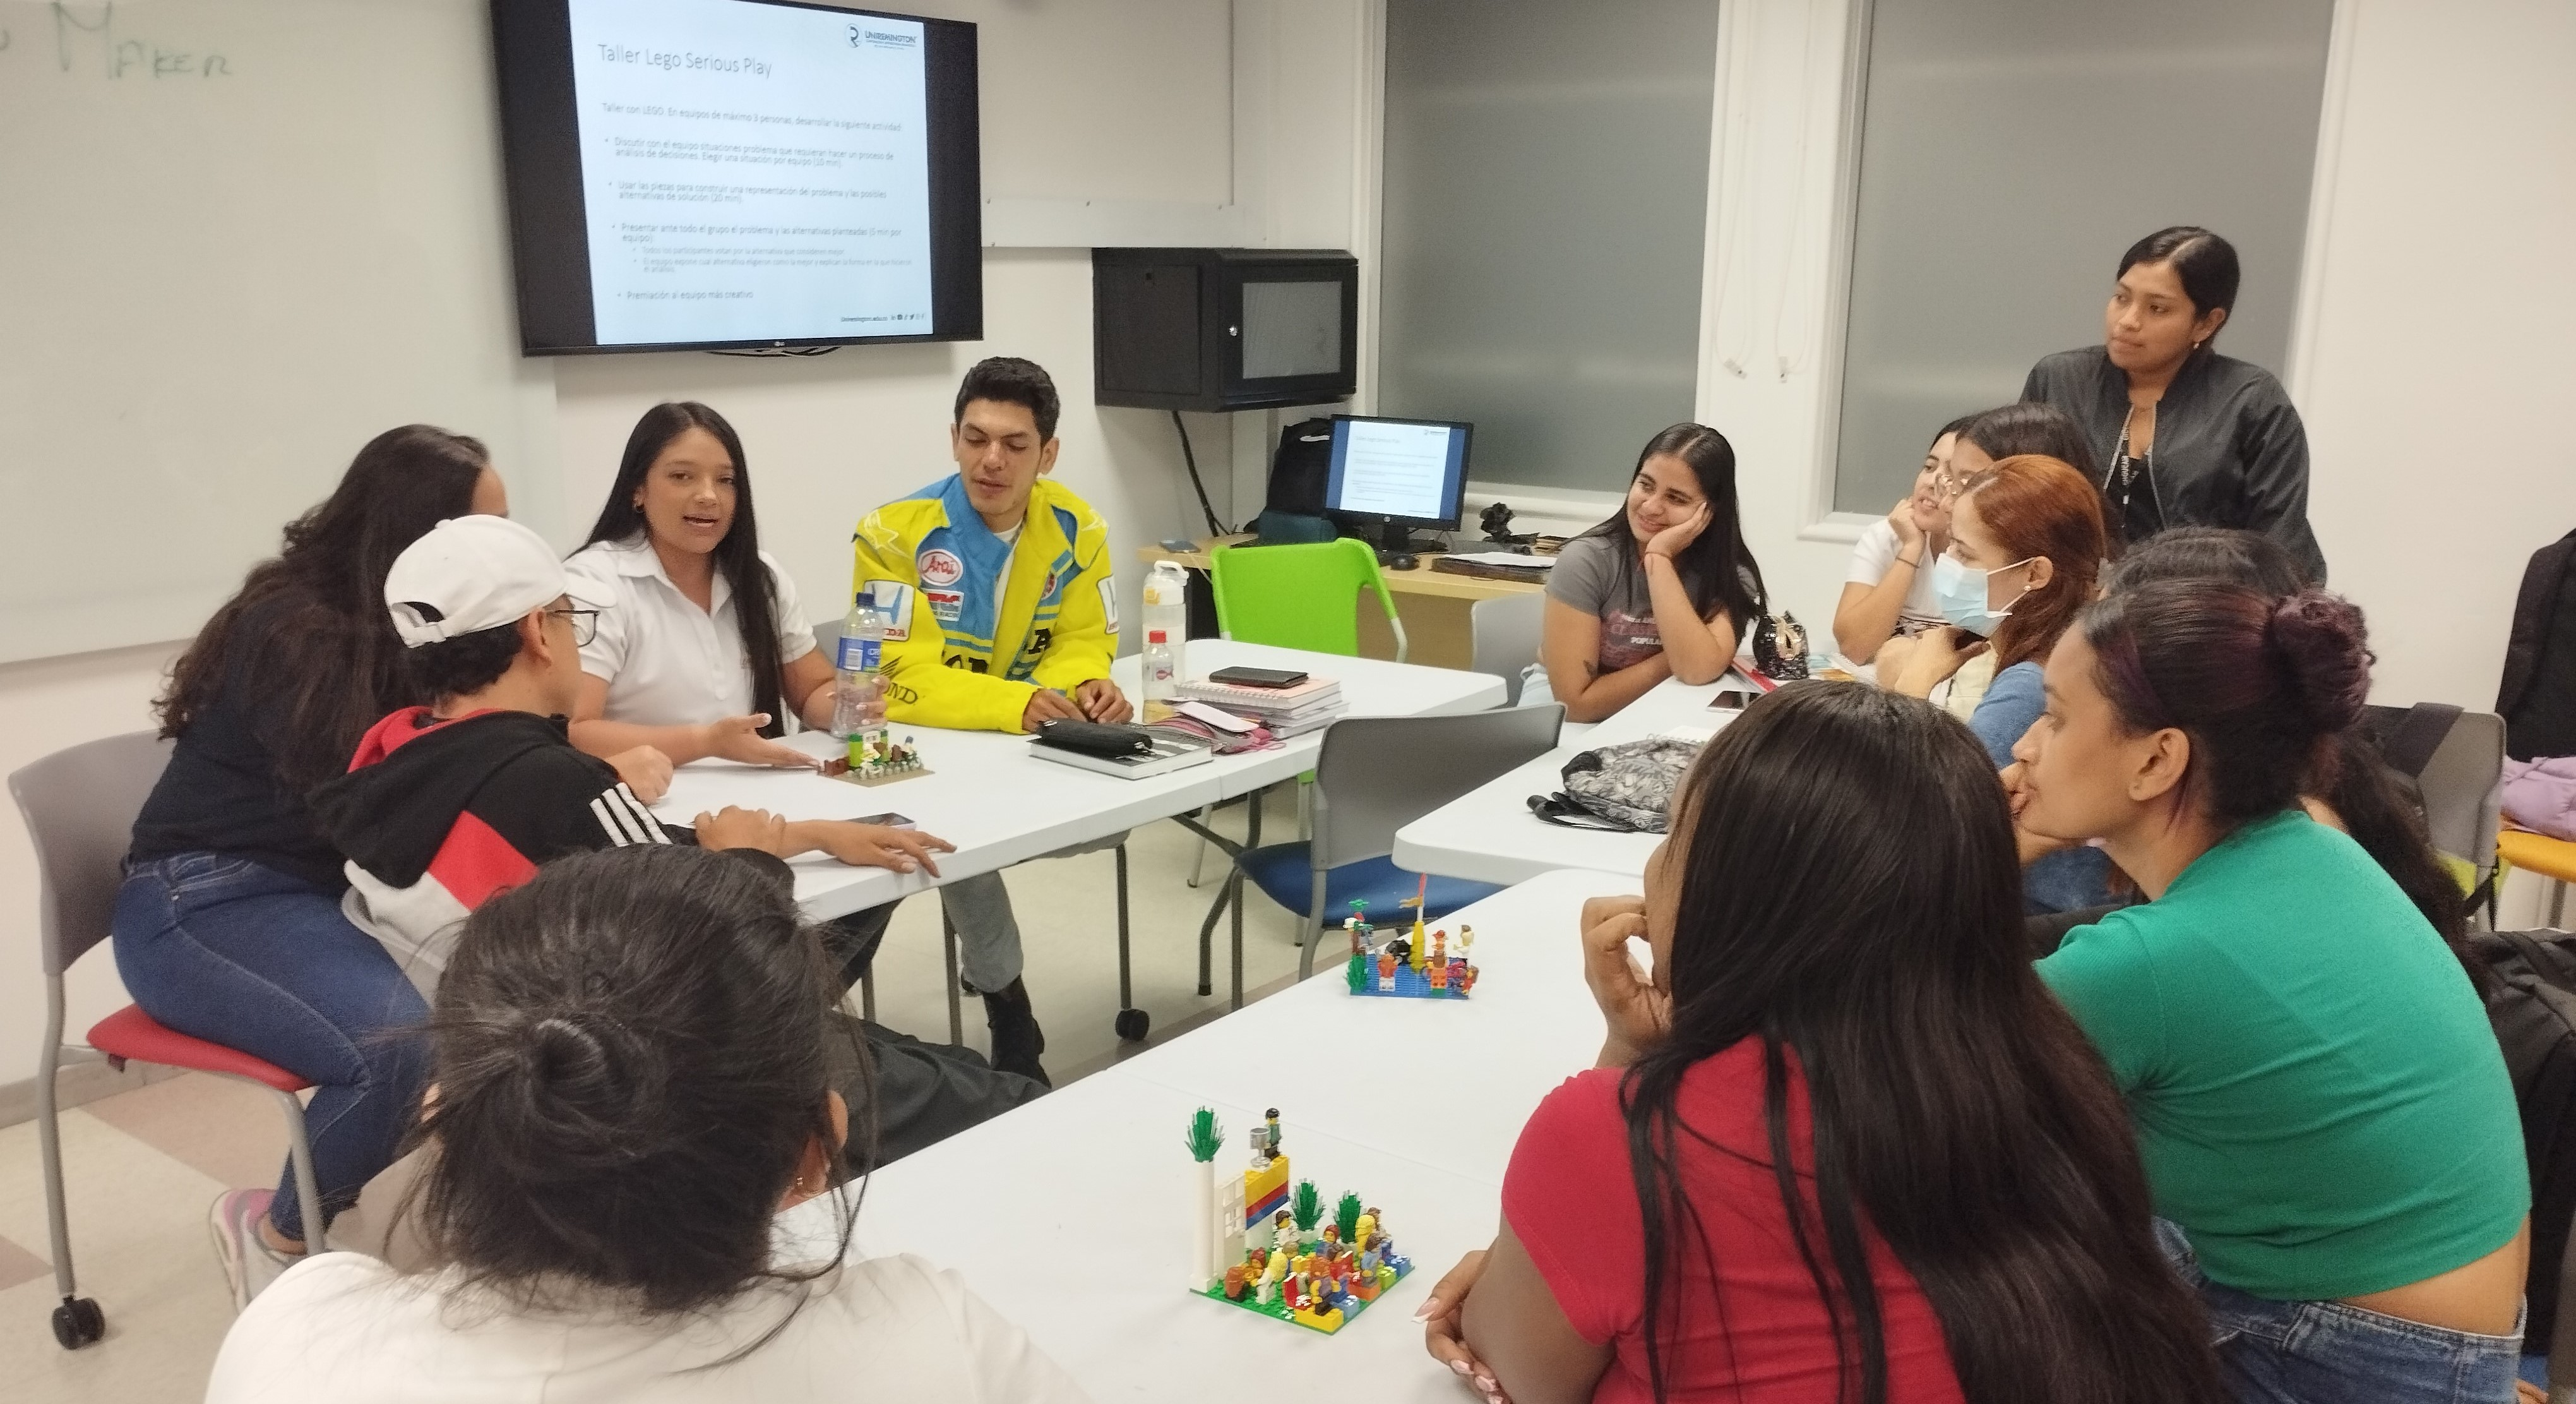
\includegraphics[width=0.15\linewidth]{students4} \end{flushleft}
\end{frame}

\begin{frame}{Getting to Know UniRemington (Students and the LEGO Lab)}
\phantomsection\label{getting-to-know-uniremington-students-and-the-lego-lab}
\begin{center}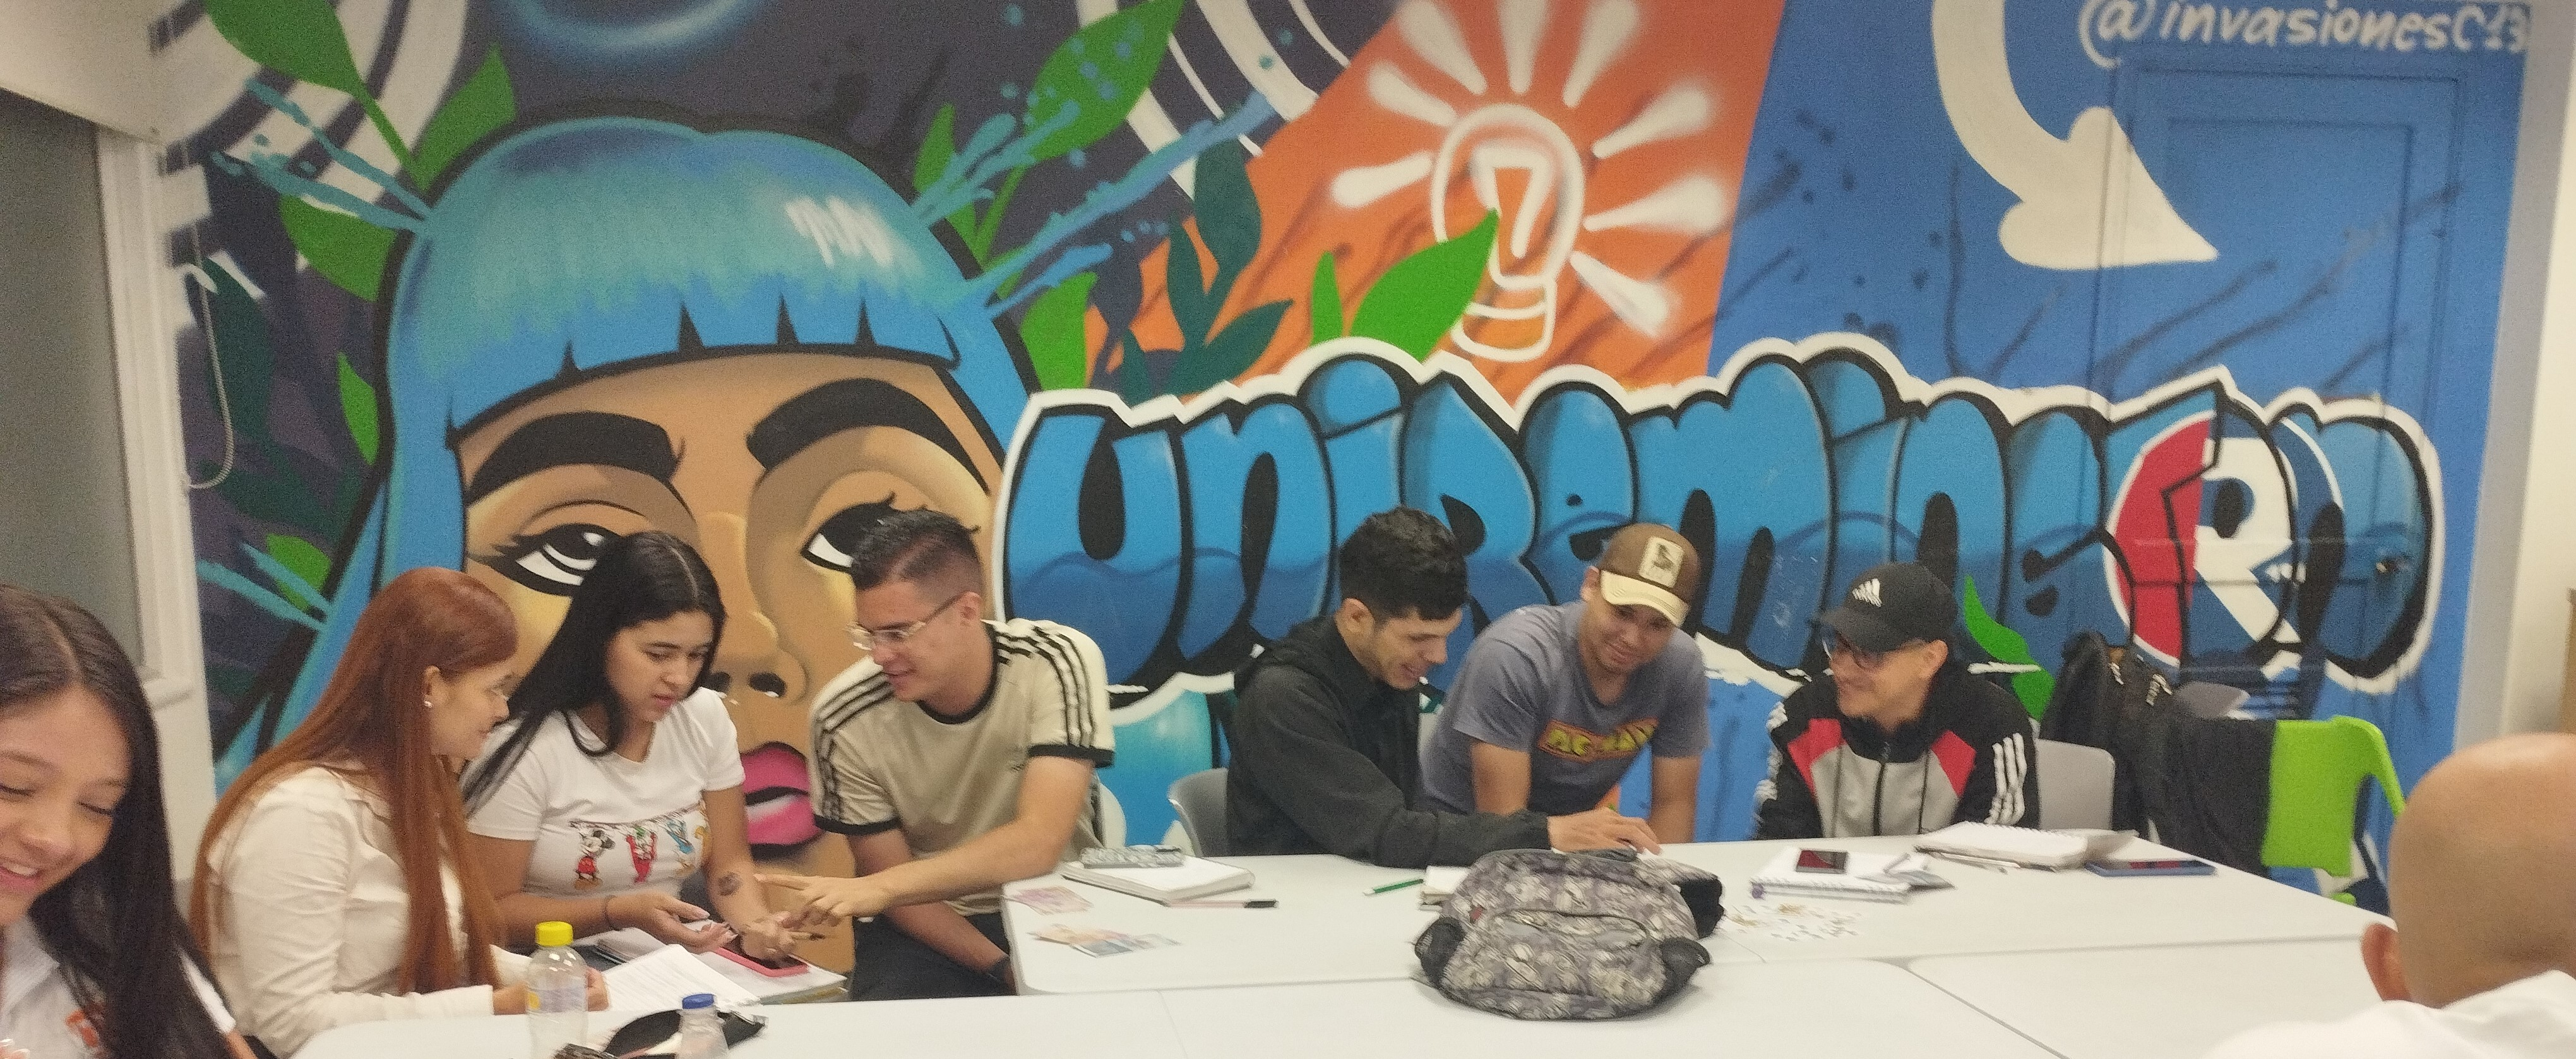
\includegraphics[width=0.3\linewidth]{students3} 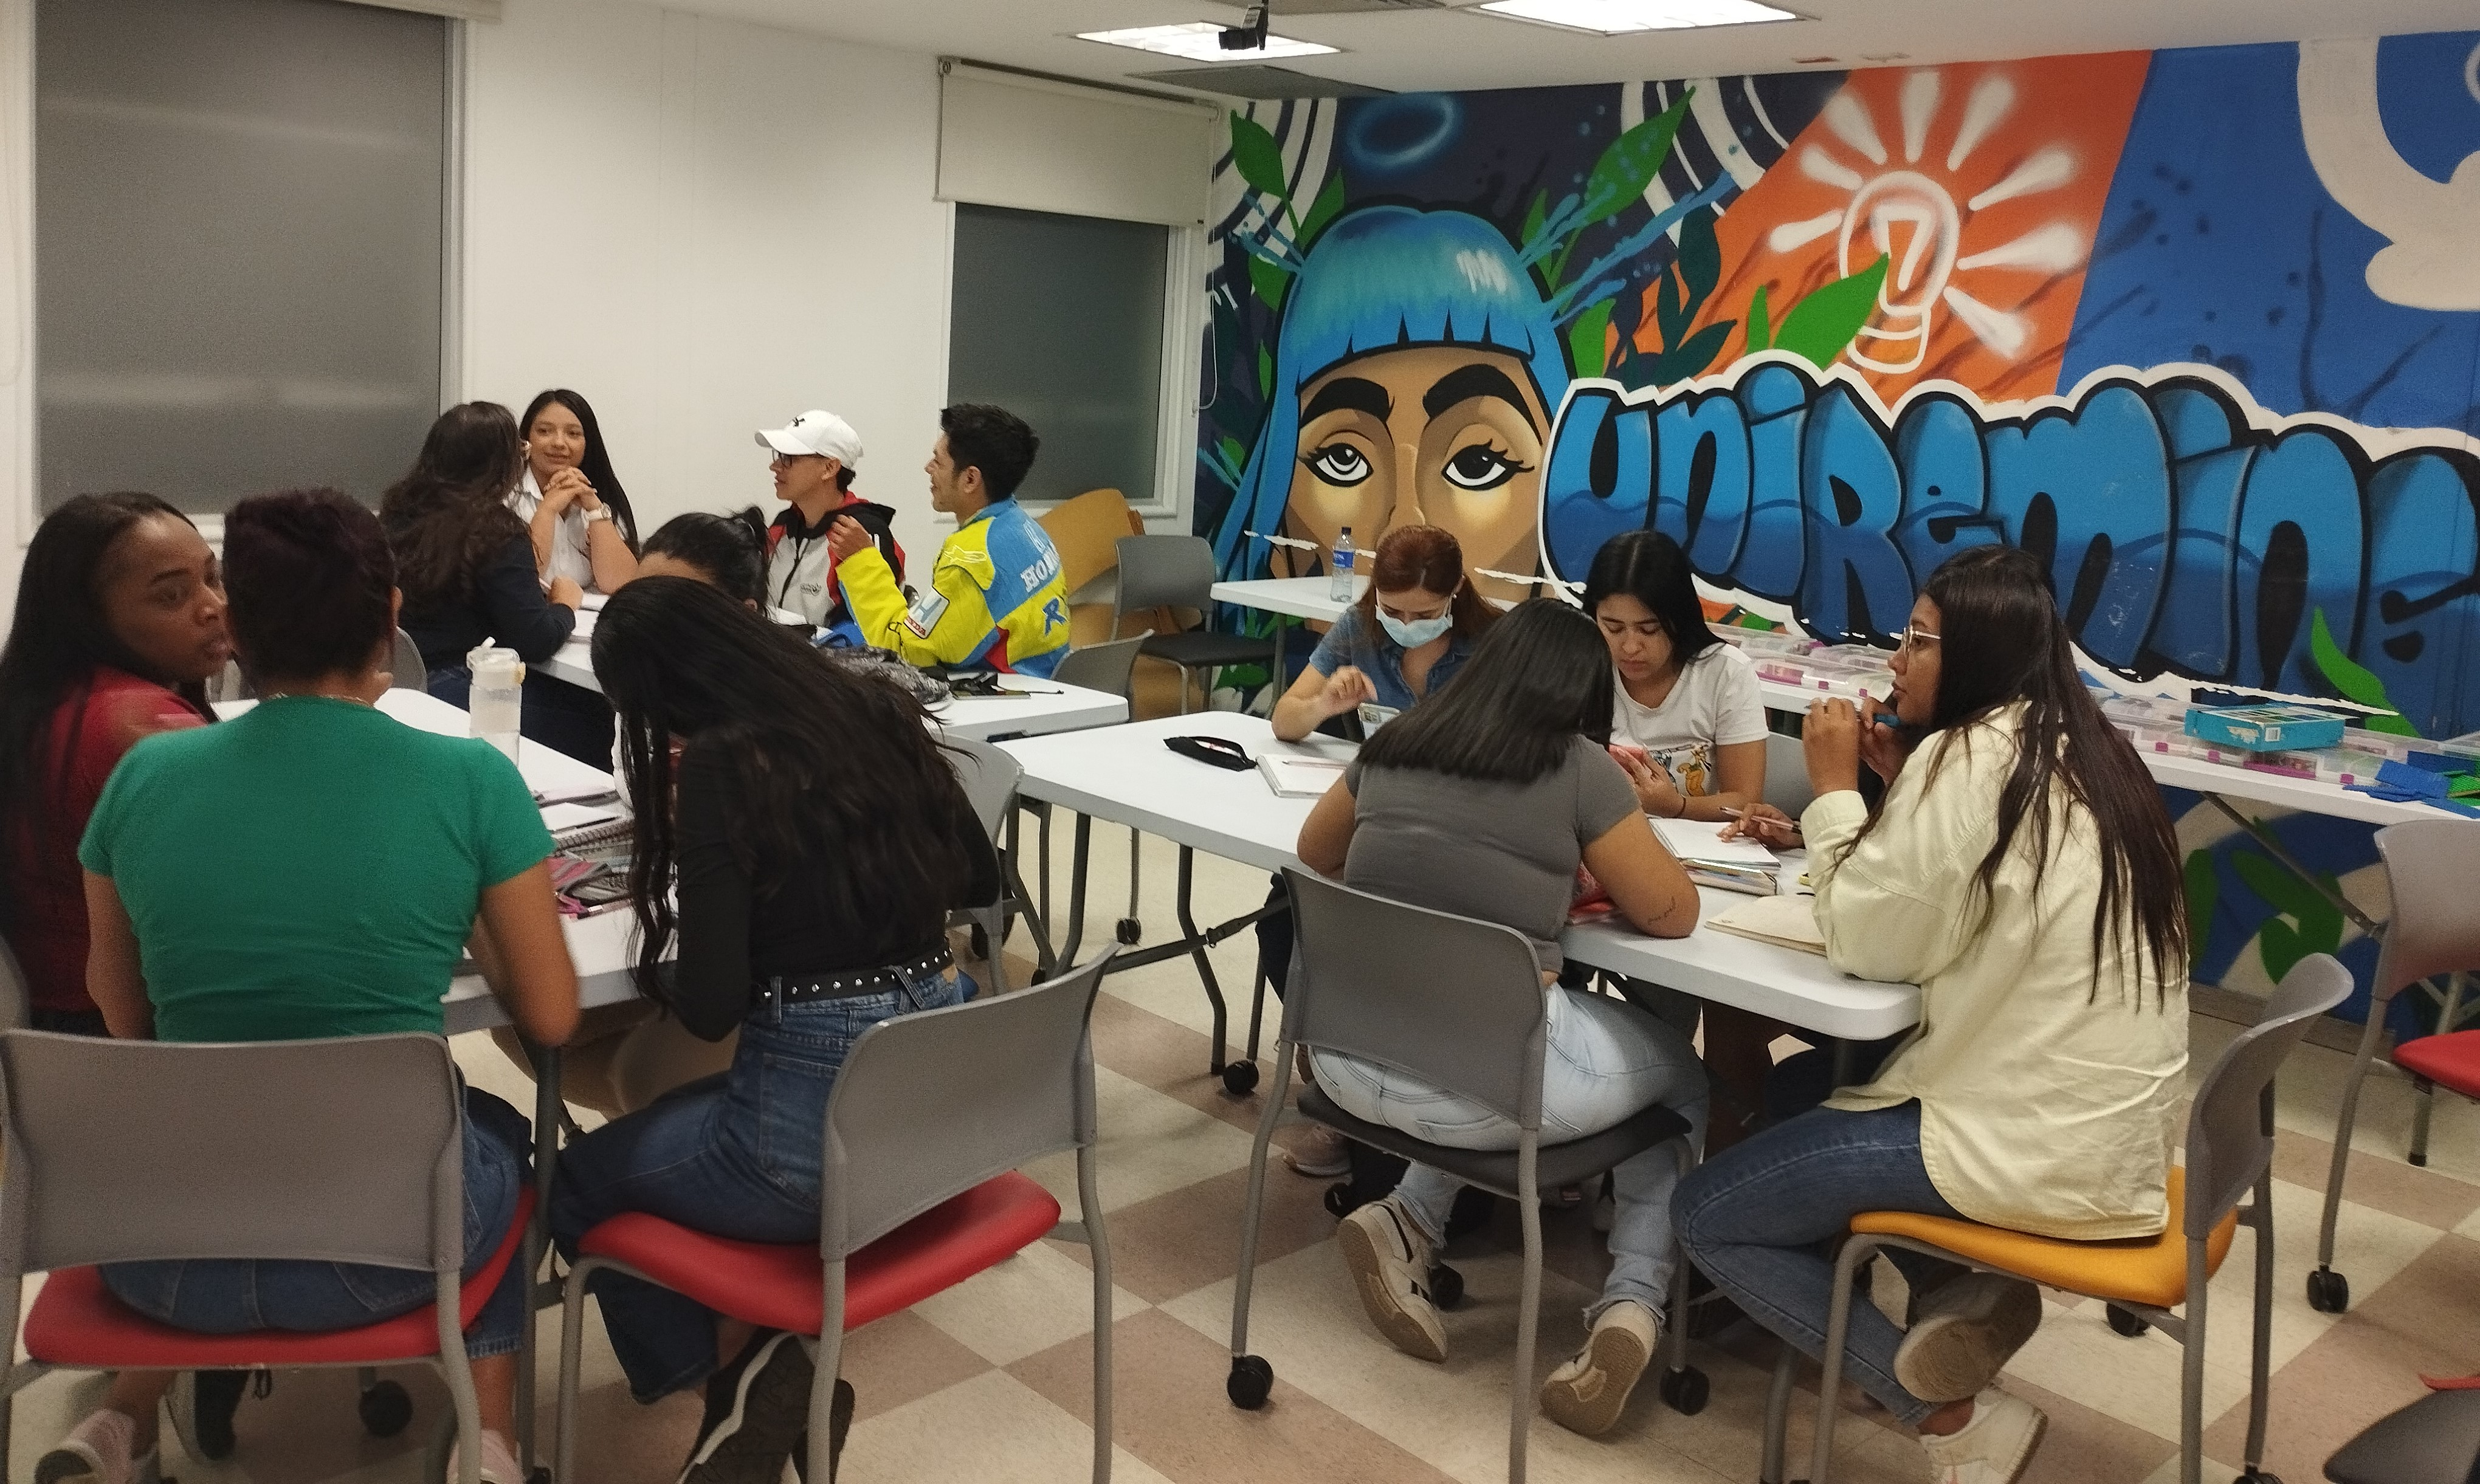
\includegraphics[width=0.3\linewidth]{students2} 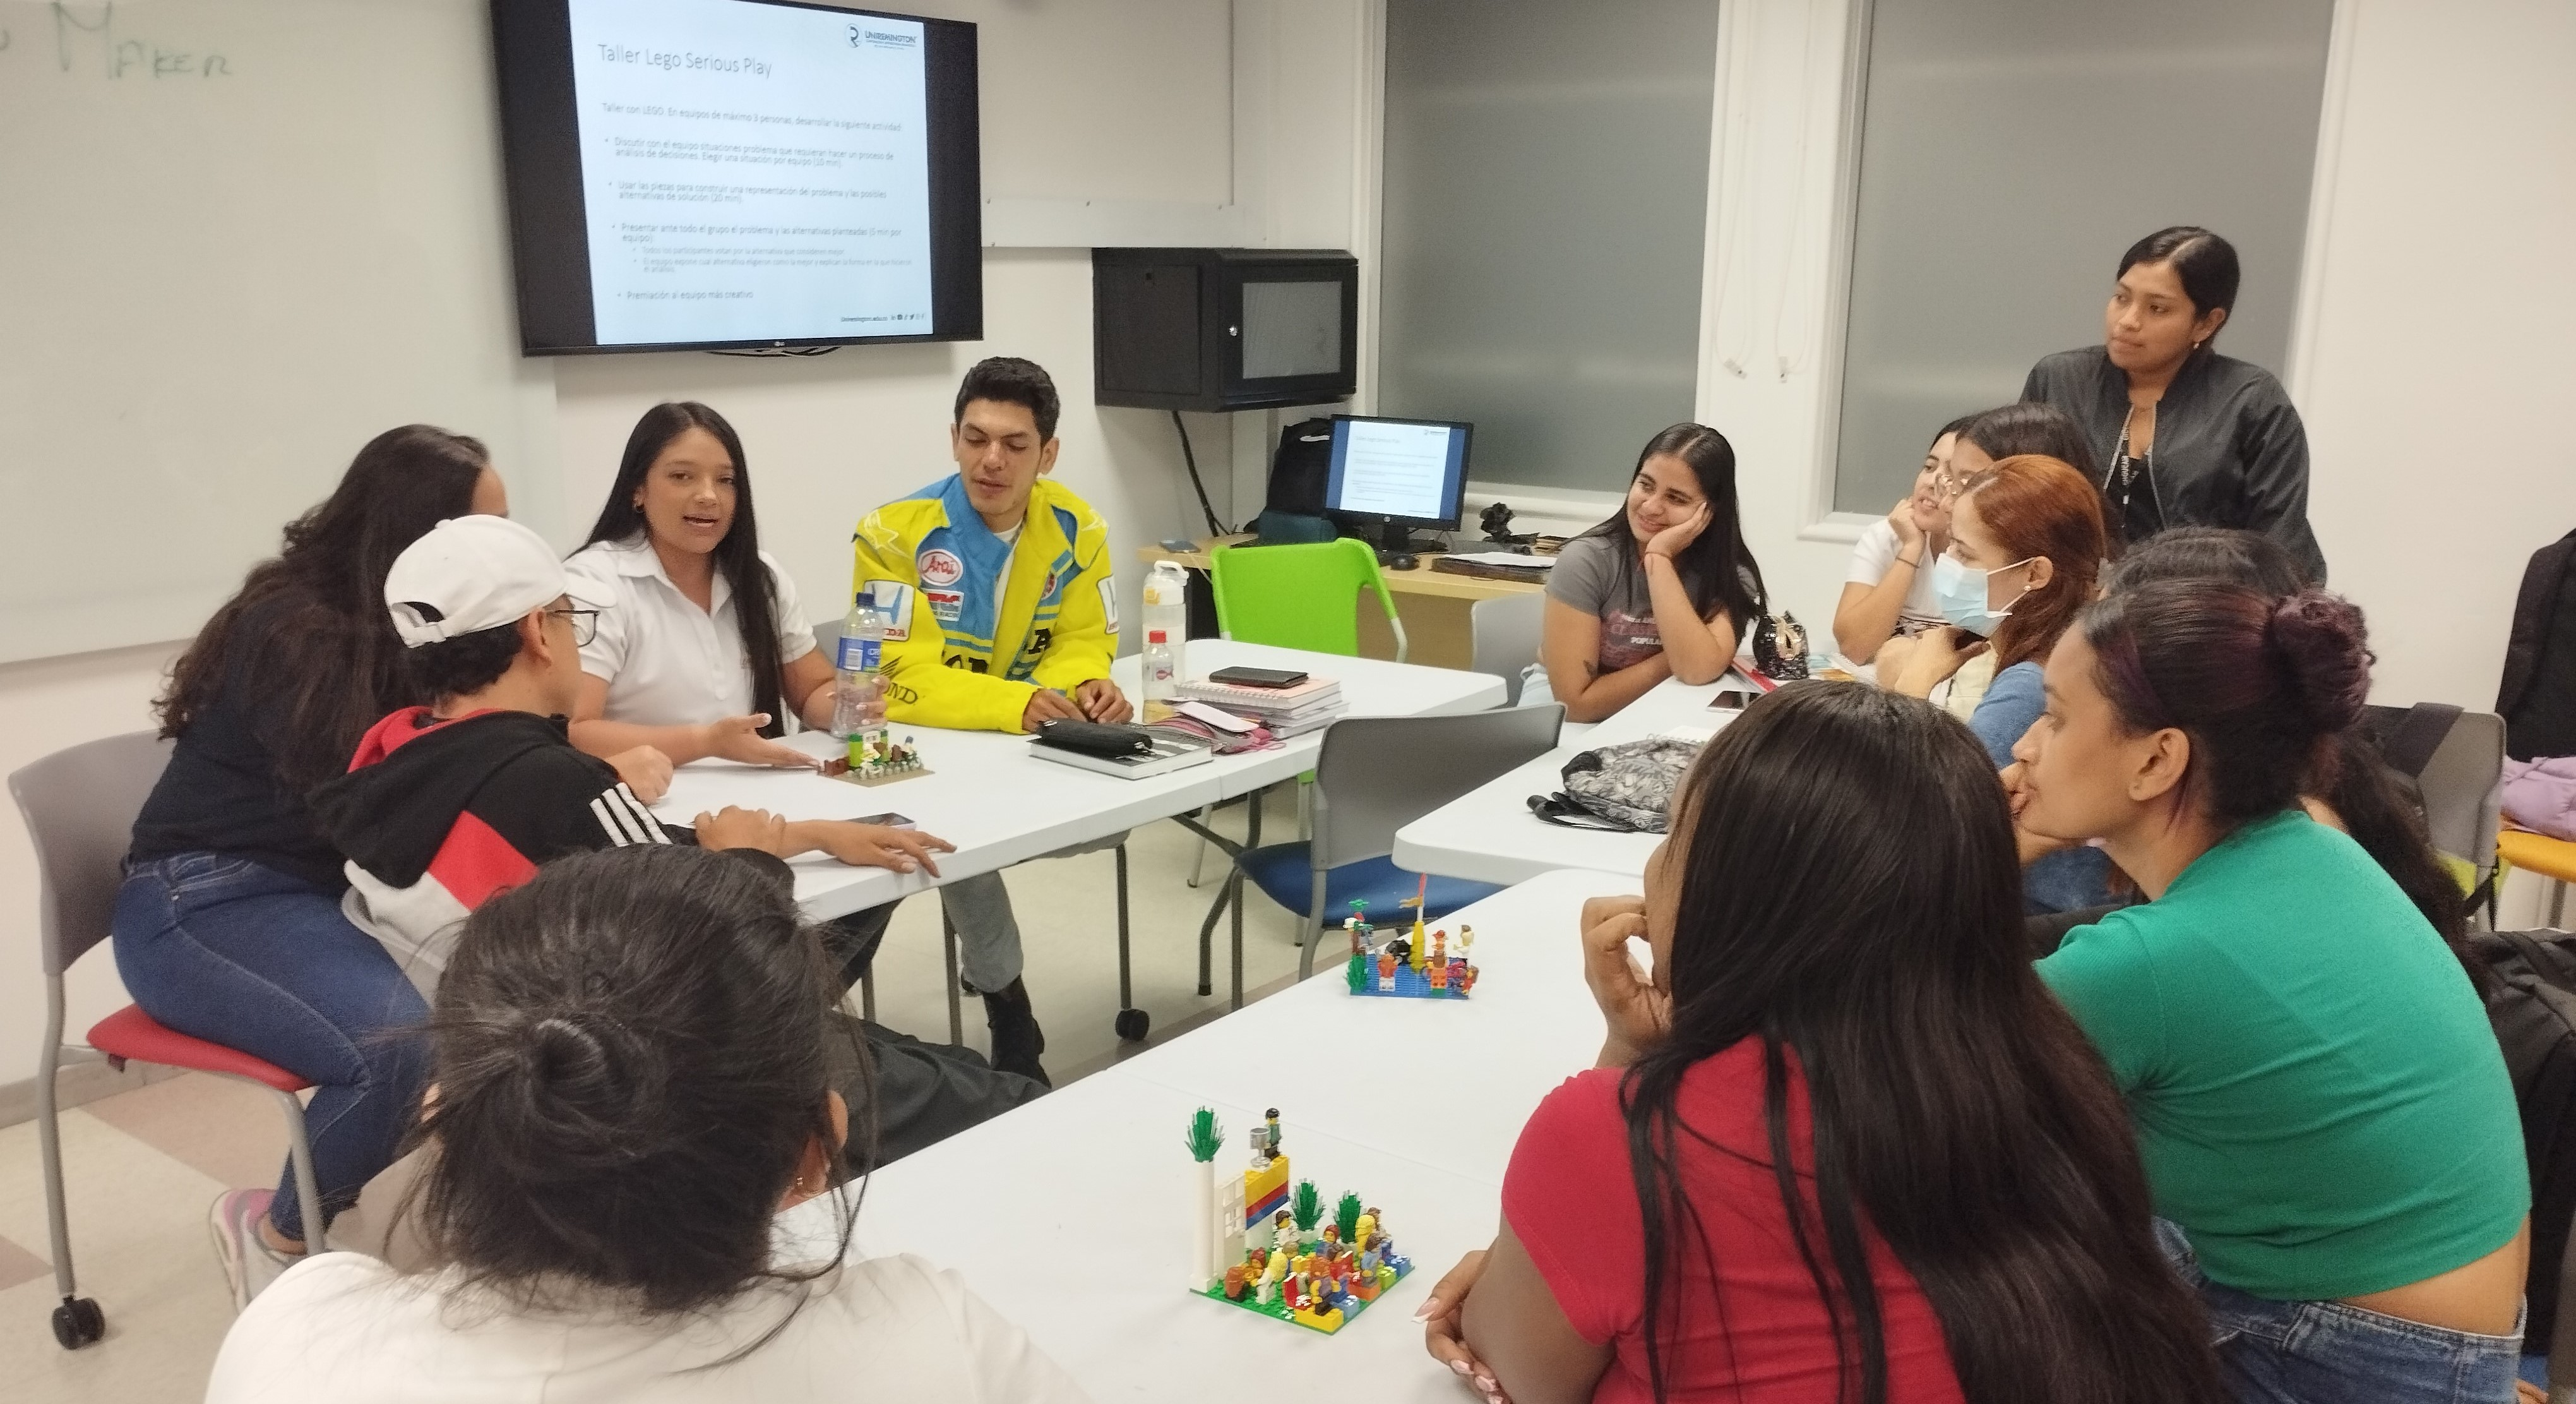
\includegraphics[width=0.3\linewidth]{students4} 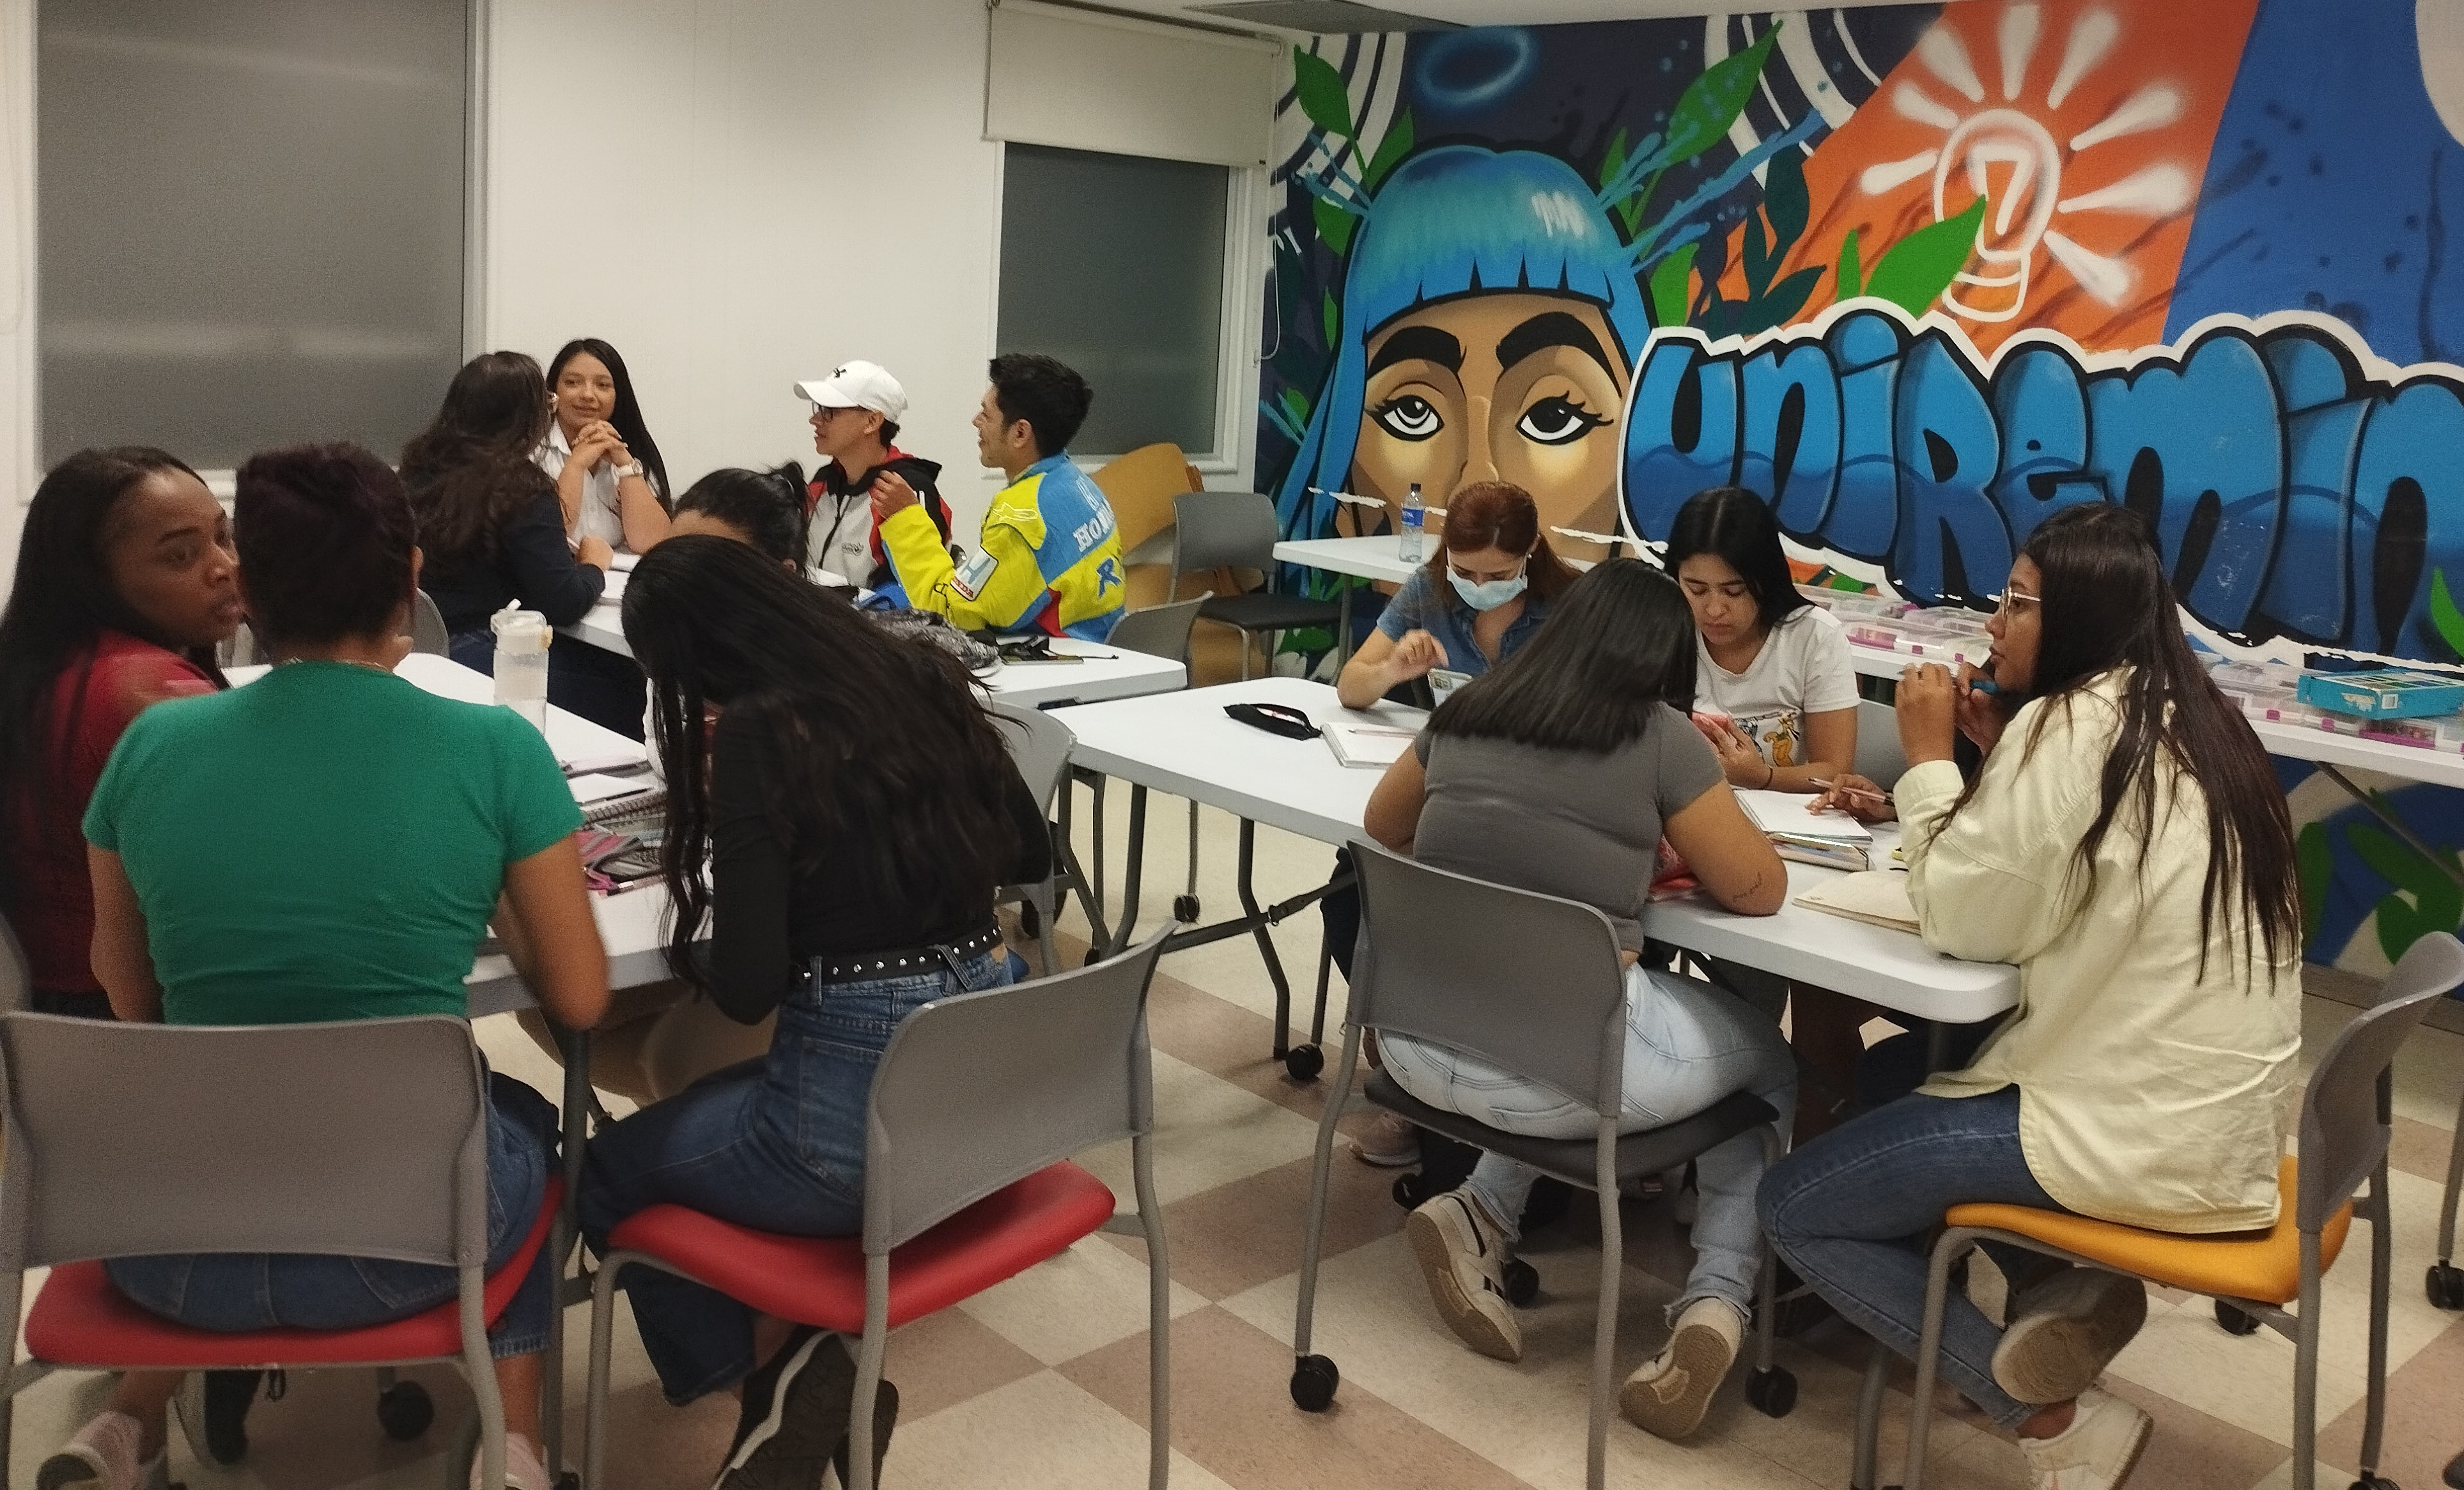
\includegraphics[width=0.3\linewidth]{students6} 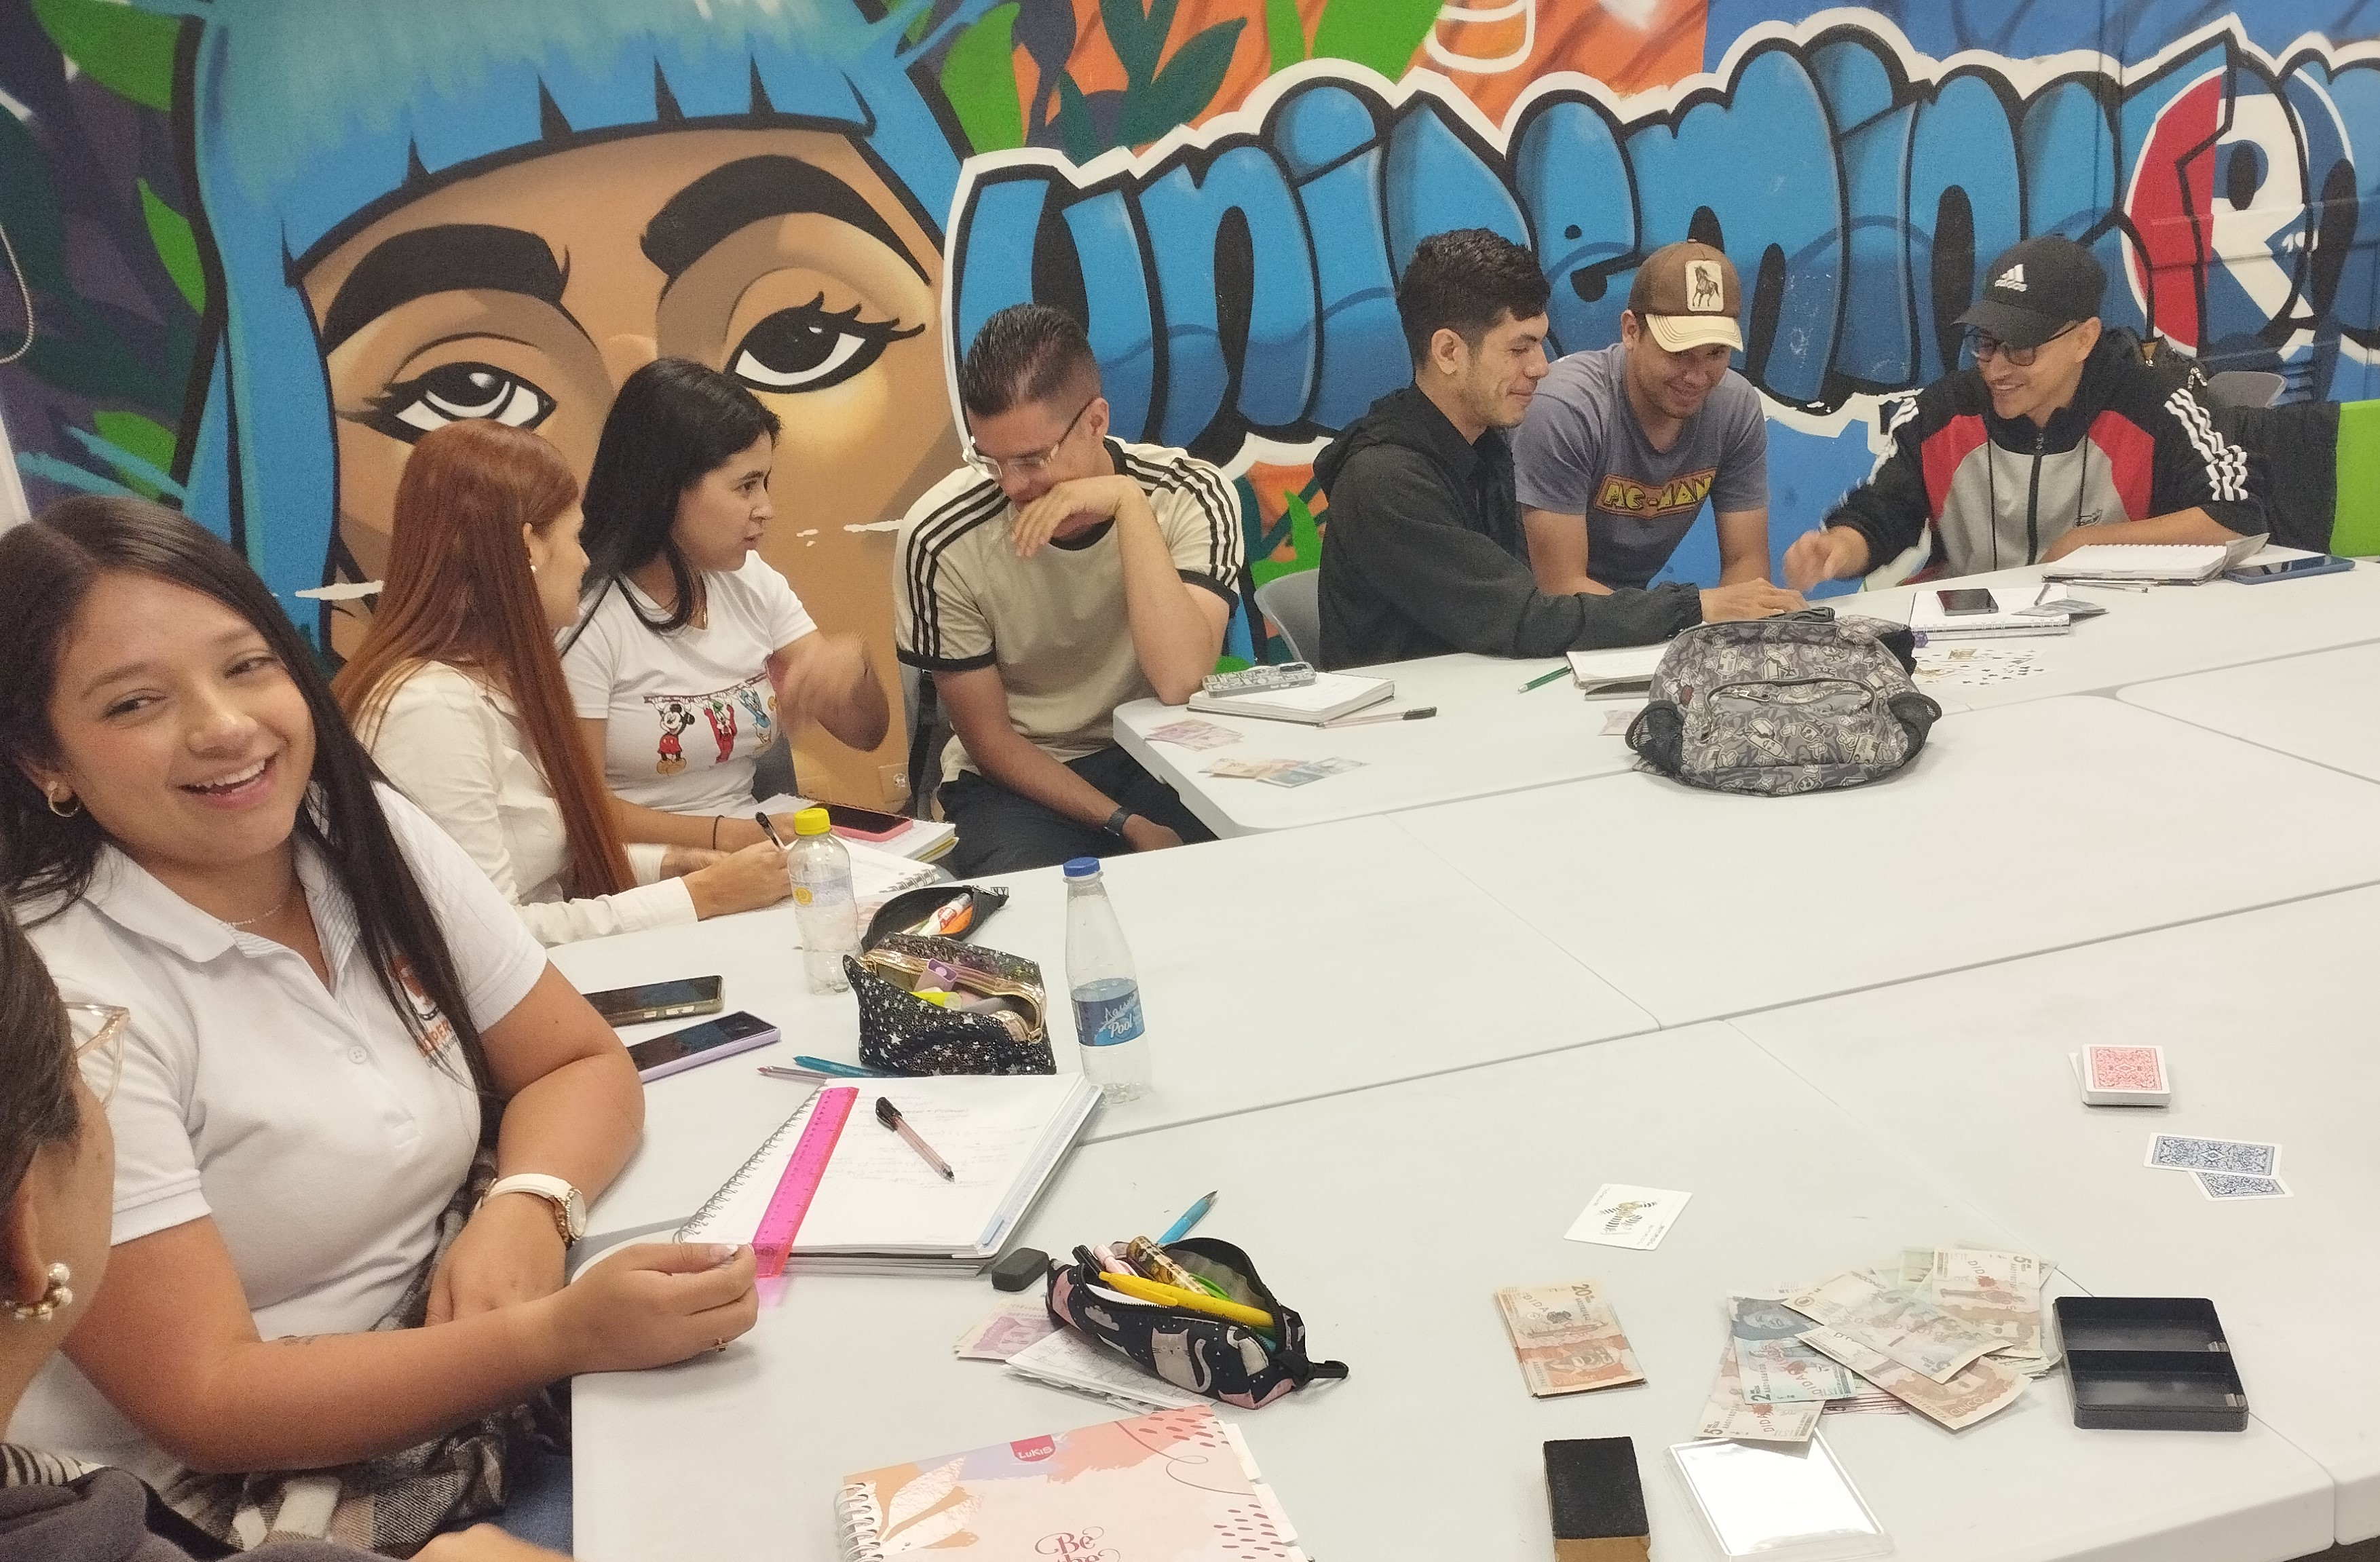
\includegraphics[width=0.3\linewidth]{students5} 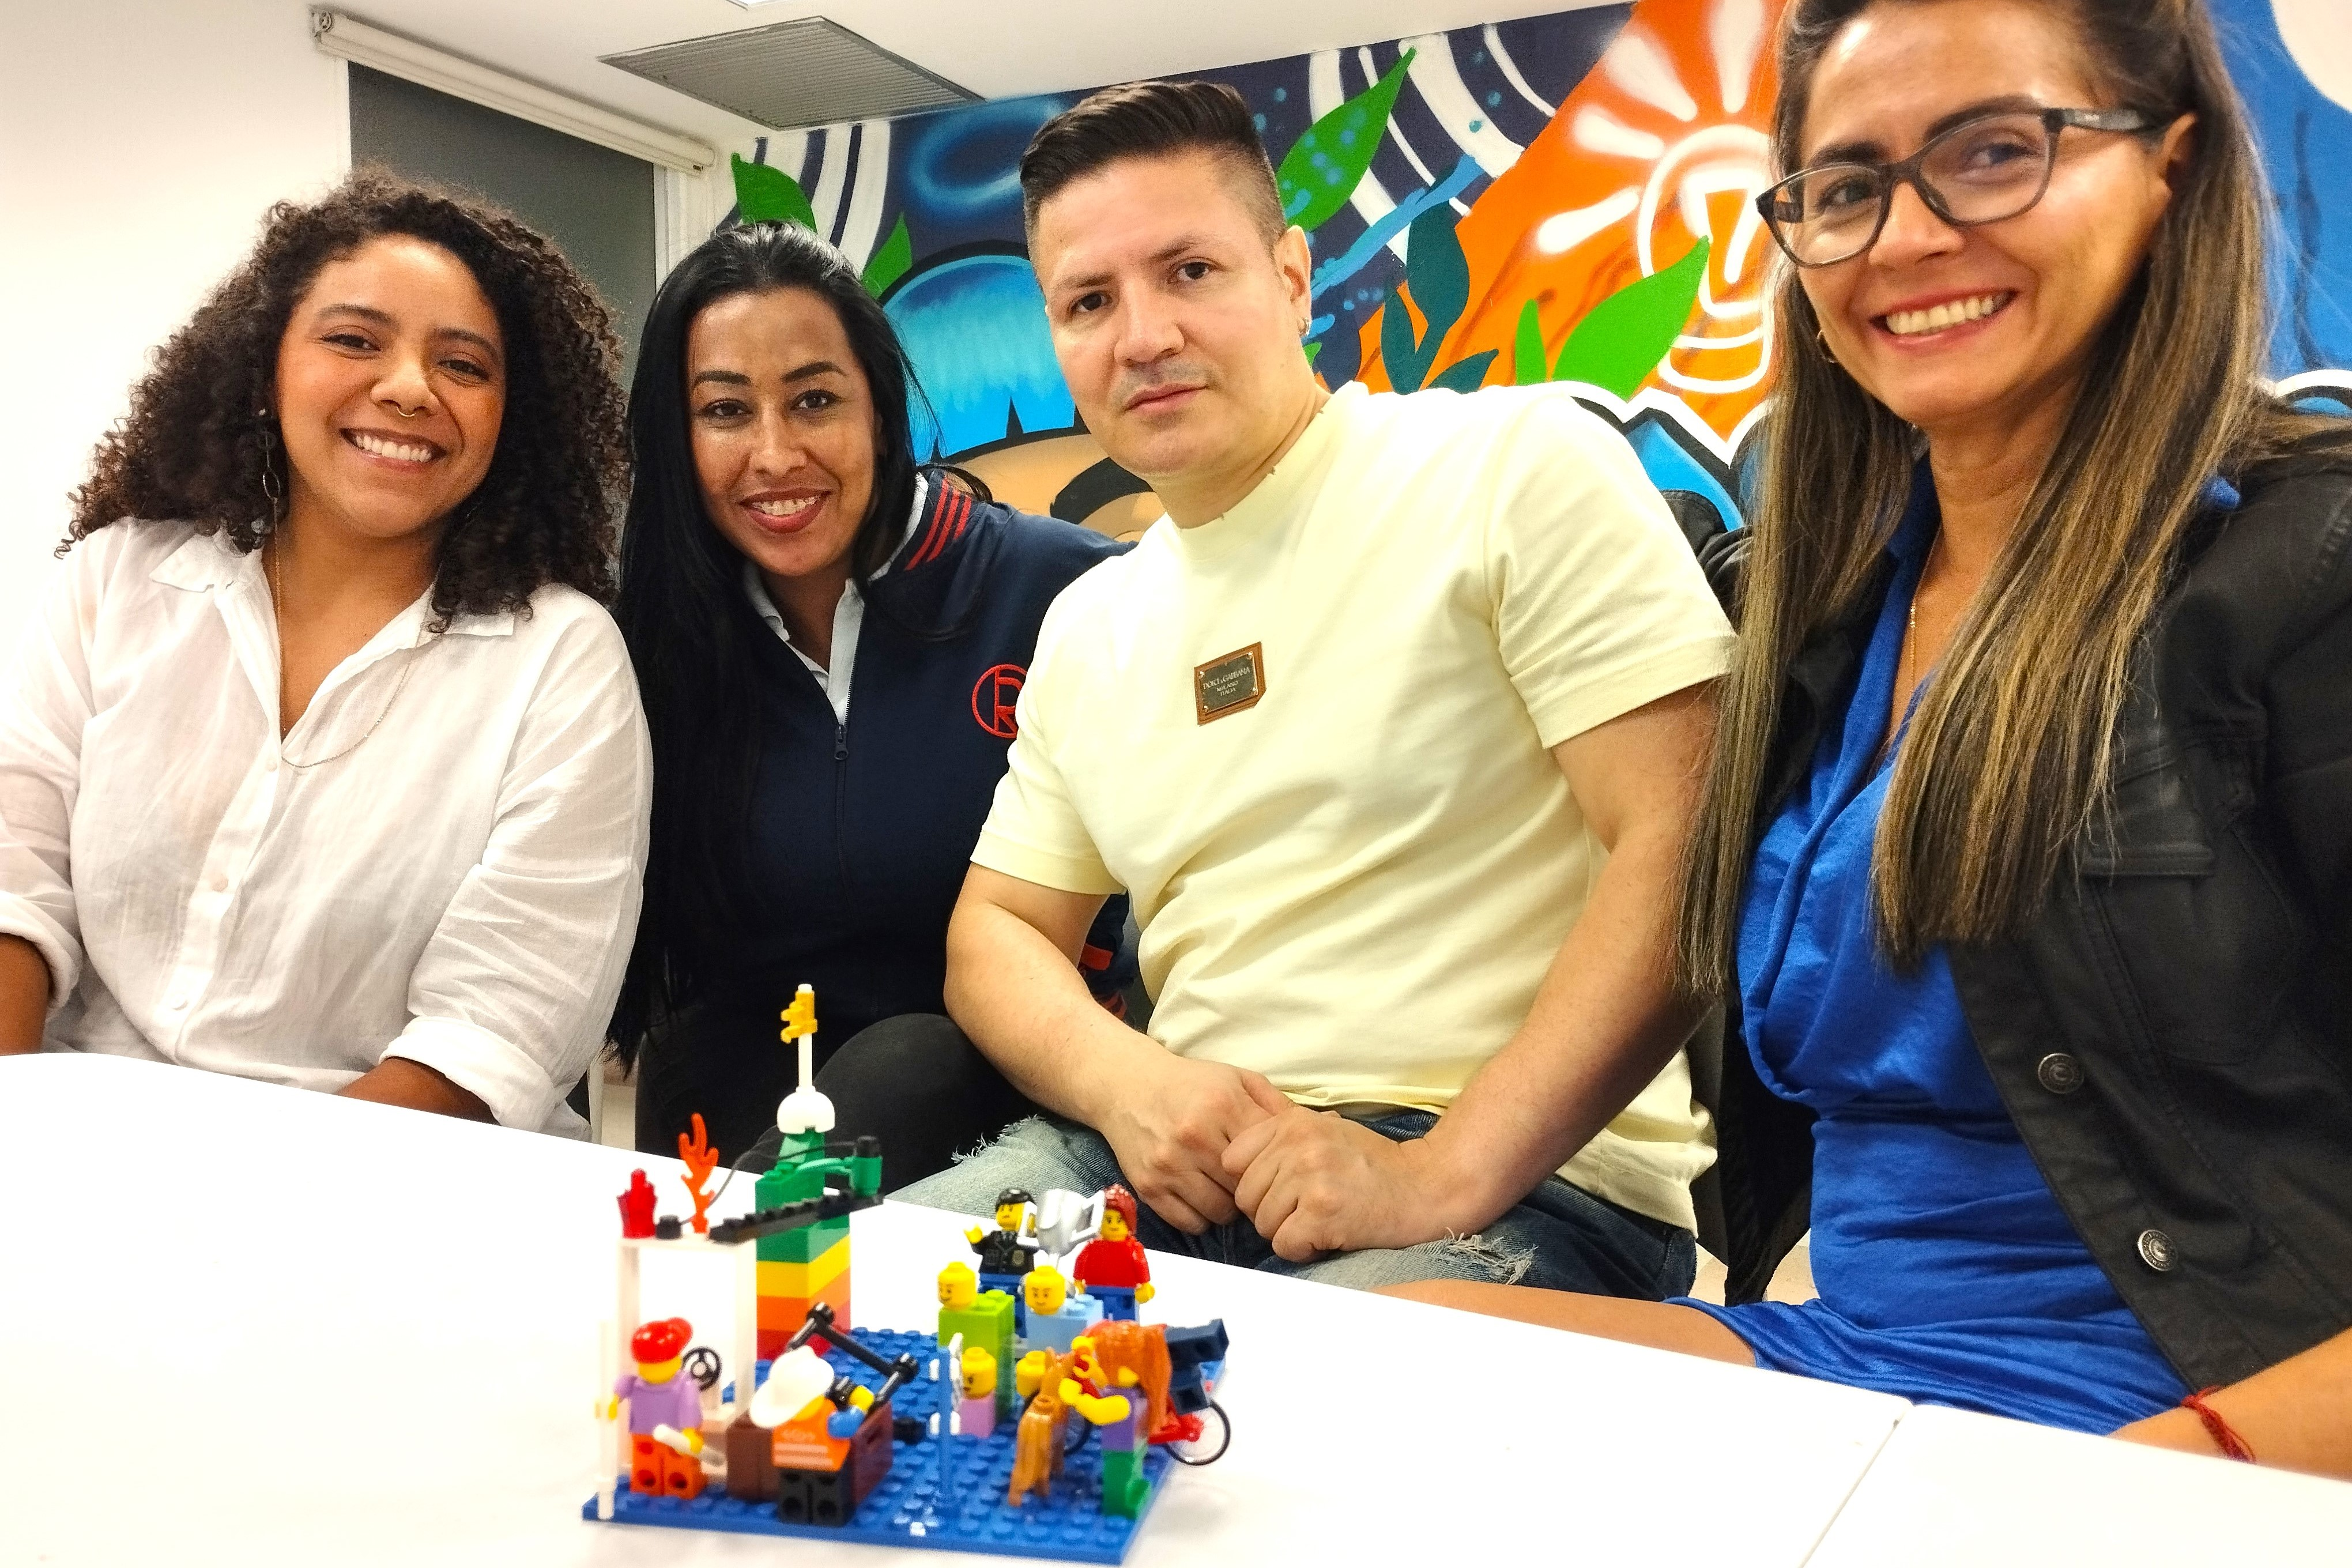
\includegraphics[width=0.3\linewidth]{students} \end{center}
\end{frame}

\begin{frame}{Getting to Know UniRemington (Faculty)}
\phantomsection\label{getting-to-know-uniremington-faculty}
\begin{center}\includegraphics[width=0.45\linewidth]{lab_collegues} \includegraphics[width=0.45\linewidth]{lunch} \end{center}
\end{frame}

\begin{frame}{Brainstorming ``Interactive Experience'' at the Escape
Room}
\phantomsection\label{brainstorming-interactive-experience-at-the-escape-room}
Escape Rooms are hugely successful games

\begin{itemize}
\tightlist
\item
  inspired by the Myst computer games of the 1990s
\item
  they are hugely popular, commercially successful and have engaged a
  wide range of audiences
\end{itemize}

They engage players in a physical environment with a sequence of time
constrained puzzles and an ultimate objective that varies with each game

\begin{flushleft}\includegraphics[width=0.45\linewidth]{escape} \end{flushleft}
\end{frame}

\begin{frame}{Brainstorming ``Interactive Experience'' at the Escape
Room}
\phantomsection\label{brainstorming-interactive-experience-at-the-escape-room-1}
Here were lessons we could learn about successfully engaging players in
an ``experience''

\begin{itemize}
\tightlist
\item
  make the challenges visceral
\item
  facilitator remote monitors and only steps in when players are
  ``stuck''
\item
  communication is via a computer monitor, players are on their own
\item
  use a sequence of short workouts / puzzles (\textless10 minutes) to
  keep interest
\end{itemize}
\end{frame}

\begin{frame}{Classroom Engagement and Protocols}
\phantomsection\label{classroom-engagement-and-protocols}
We asked ``What can we do with a course to create an exciting and
engaging student \emph{`interactive experience'}?''

In collaboration with the faculty, we decided to prototype the creation
of ``interactive experiences'' using the Innovation \& Creativity Lab
supporting three different 2-hour classes:

\begin{itemize}
\tightlist
\item
  Marketing mix and strategy
\item
  Colombian Economy and flows of money
\item
  Portfolio management
\end{itemize}

These selections cover a diverse set of topics assuring a wide buy-in by
university faculty
\end{frame}

\begin{frame}{Class 1: Marketing Mix Class}
\phantomsection\label{class-1-marketing-mix-class}
\small

Objective: Learn how to achieve an optimal \emph{Marketing Mix} with
LEGO integration:

Class Overview:

\begin{itemize}
\tightlist
\item
  Format: In-person, synchronous (i.e., all at the same time, same
  place) two-hour interactive session.
\item
  Flow: Introduction and setup, followed by six decision-making rounds
  on product, price, place, and promotion in the marketing mix.
\item
  Reflection: Post-round reflections and a final session for grading and
  real-world insights into market dynamics and strategic decisions.
\end{itemize}
\end{frame}

\begin{frame}{Class 1: Marketing Mix Class}
\phantomsection\label{class-1-marketing-mix-class-1}
\small

Enhancements from Escape Room Insights:

\begin{itemize}
\tightlist
\item
  Facilitator's Role: Subtle guidance to keep participants engaged and
  productive.
\item
  Group Size: Ideal groups of five for balance between individual
  participation and teamwork.
\item
  Task Segmentation: Short, sequential tasks for progressive learning
  and focus.
\item
  Physical Space: Defined work zones to enhance focus and teamwork.
\end{itemize}

\begin{flushleft}\includegraphics[width=0.3\linewidth]{lego} \end{flushleft}
\end{frame}

\begin{frame}{Class 1: Marketing Mix Class}
\phantomsection\label{class-1-marketing-mix-class-2}
\small

Engagement Techniques:

\begin{itemize}
\tightlist
\item
  Instructions \& Cues: Clear verbal instructions with timed
  visual/auditory cues for responsiveness.
\item
  Monitoring \& Feedback: Remote monitoring with digital feedback for
  autonomy and support.
\item
  Timed Hints: Scheduled cues to ensure critical information is
  retained, boosting engagement.
\end{itemize}

Goal: Create a simulation that is interactive, effective, and fosters
deep learning through hands-on engagement and teamwork.

\begin{flushleft}\includegraphics[width=0.3\linewidth]{lego} \end{flushleft}
\end{frame}

\begin{frame}{Class 2: The Colombian Economy and Flows of Money}
\phantomsection\label{class-2-the-colombian-economy-and-flows-of-money}
\small

Class Overview:

\begin{itemize}
\tightlist
\item
  Format: In-person, two-hour interactive session.
\item
  Flow: Student briefing and simulation setup, followed by six
  decision-making rounds where each institution (bank, government,
  consumers, industry) pursues its unique goals and philosophy, all of
  which influence their control over monetary policy and flows
\item
  Reflection: Post-round reflections and a final session for grading and
  real-world insights into decisions that helped or hurt the Colombian
  economy, industry, and households
\end{itemize}

\begin{flushleft}\includegraphics[width=0.5\linewidth]{economy} \end{flushleft}
\end{frame}

\begin{frame}{Class 2: Colombian Economy and Flows of Money Class}
\phantomsection\label{class-2-colombian-economy-and-flows-of-money-class}
\small

Sequence of Workout Tasks for Colombian Economy and Flows of Money
Class:

Introduction (10 min): Outline objectives, simulation mechanics, and
setup instructions.

Challenge Rounds (6 rounds, 15 min each):

\begin{itemize}
\tightlist
\item
  Provide simulated currency (fake bills or LEGO pieces) to students.
\item
  Students represent roles in the economy (government, central bank,
  households, industry).
\item
  Groups of four compete based on their chosen economic philosophy.
\item
  Event Presentation (1 min): Up to five random events are introduced,
  impacting each group differently based on their economic philosophy.
\end{itemize}
\end{frame}

\begin{frame}{Class 2: Colombian Economy and Flows of Money Class}
\phantomsection\label{class-2-colombian-economy-and-flows-of-money-class-1}
\small

Active Play (10 min): Students adjust money flows with LEGO tokens and
bills according to event impacts.

Reflection (5 min): Groups evaluate decisions and develop strategies for
the next round.

Final Reflection (15 min): Group discussion on strategies, patterns
observed, and learning outcomes.

Self-Grading and Evaluation: Groups assess each others' success in
managing the Colombian economy.

Teacher Evaluation: The teacher grades each group on ultimate simulated
GDP, per capita wealth, industrial output, and tax revenues.
\end{frame}

\begin{frame}{Class 3: Portfolio Management Class Designed for
Scalability}
\phantomsection\label{class-3-portfolio-management-class-designed-for-scalability}
\small

\textbf{\href{https://github.com/westland/Fulbright/blob/main/portfolio_mngt_virtual_class.pdf}{Virtual
Classroom Challenge - Instructions}}

Format of Asynchronous Portfolio Management Class: Virtual, fully
automated, accessible 24/7

Structure:

\begin{itemize}
\tightlist
\item
  Introduction and Setup: Overview of objectives and app mechanics.
\item
  Interactive Rounds: Six rounds where students analyze event impacts,
  adjust investments, and receive immediate grading.
\item
  Reflection: Post-round reflection for strategic insights.
\item
  Performance Incentives: Leaderboard and grading curve to motivate
  students.
\item
  Final reflections and Grading
\end{itemize}
\end{frame}

\begin{frame}{Class 3: Portfolio Management Class Designed for
Scalability}
\phantomsection\label{class-3-portfolio-management-class-designed-for-scalability-1}
\small

Applying Escape Room Protocols: To enhance simulation experiences,
fostering engagement, teamwork, and effective learning

\begin{itemize}
\tightlist
\item
  Facilitator's Role: Not necessary, but where used, subtle guidance to
  maintain engagement and productivity.
\item
  Task Segmentation: Short, sequential tasks for focused learning.
\item
  Physical Space: None needed
\item
  Monitoring \& Feedback: Remote progress tracking with digital feedback
  to encourage autonomy.
\item
  Timed Hints: Cues to highlight critical information, boosting
  engagement and responsiveness.
\end{itemize}
\end{frame}

\begin{frame}{Class 3: Portfolio Management Class Designed for
Scalability}
\phantomsection\label{class-3-portfolio-management-class-designed-for-scalability-2}
\small

\textbf{\href{https://jcwestland.shinyapps.io/virtual_invest_class/}{Virtual
Classroom Challenge - Software}}

Summary of sequence of workout tasks for the Portfolio Management class:

\begin{itemize}
\tightlist
\item
  Introduction (10 minutes): Overview of objectives, simulation
  mechanics, and setup.
\item
  Challenge Rounds (6 rounds, 15 minutes each) and Event Presentation:
  Up to 5 random events impact specific securities.
\item
  Active Play (10 minutes): Students adjust holdings using sliders based
  on event impacts.
\item
  Reflection (5 minutes): Evaluate decisions, strategize for the next
  round..
\item
  Automatic grading based on portfolio value, risk management, and
  strategic consistency.
\end{itemize}
\end{frame}

\begin{frame}{Investment in Colombia's Future: Experiential,
Asynchronous, Automated}
\phantomsection\label{investment-in-colombias-future-experiential-asynchronous-automated}
\small

\textbf{Unlocks Potential of a Young, Energetic Workforce:} Colombia's
youthful population holds enormous potential to drive economic growth,
but they need access to relevant, high-quality education tailored to
modern industry needs.

\textbf{Bridges the Teacher Gap in Tech-Centric Fields:} With a shortage
of educators trained in current tech and industry practices, automated,
self-paced courses can scale high-demand knowledge to thousands without
overwhelming the teaching workforce.

\textbf{Expands Access Amid Limited Institutional Capacity:} Colombia's
educational institutions face capacity constraints, making it
challenging to meet the training demands of emerging industries.
Asynchronous courses allow students to learn on their own schedule,
overcoming space and resource limitations.
\end{frame}

\begin{frame}{Investment in Colombia's Future: Experiential,
Asynchronous, Automated}
\phantomsection\label{investment-in-colombias-future-experiential-asynchronous-automated-1}
\small

\textbf{Prepares for the Global Shift in Job Markets:} Rapid changes in
the global economy, such as automation, data-driven decision-making, and
digital services, are reshaping the job landscape. These courses provide
skills for the future, ensuring Colombia's youth can compete on the
international stage.

\textbf{Fuels Economic Dynamism and Export Capacity:} A workforce
skilled in tech and industry-relevant fields empowers Colombia to
diversify its economy, boost exports, and elevate its presence in the
global market, contributing to sustainable national growth.
\end{frame}

\begin{frame}{Investment in Colombia's Future: Experiential,
Asynchronous, Automated}
\phantomsection\label{investment-in-colombias-future-experiential-asynchronous-automated-2}
\small

\textbf{Equips Colombia to be a Regional Leader:} By fostering a
well-prepared, tech-savvy workforce, Colombia can not only support its
own economy but also become a leader in Latin America, attracting
investments, talent, and innovation from around the world.

\textbf{Supports Lifelong Learning and Economic Resilience:} With
continuous access to industry-relevant knowledge, Colombians can adapt
to evolving industries over their careers, creating a resilient
workforce prepared to pivot as new opportunities emerge.

\textbf{Investing in these courses is more than education; it's a
strategy for long-term economic strength and global influence.}
\end{frame}

\begin{frame}{It wasn't all work: Discovering Colombia}
\phantomsection\label{it-wasnt-all-work-discovering-colombia}
\begin{center}\includegraphics[width=0.15\linewidth]{boterro1} \includegraphics[width=0.15\linewidth]{fruit} \includegraphics[width=0.15\linewidth]{guatape} \includegraphics[width=0.15\linewidth]{medellin} 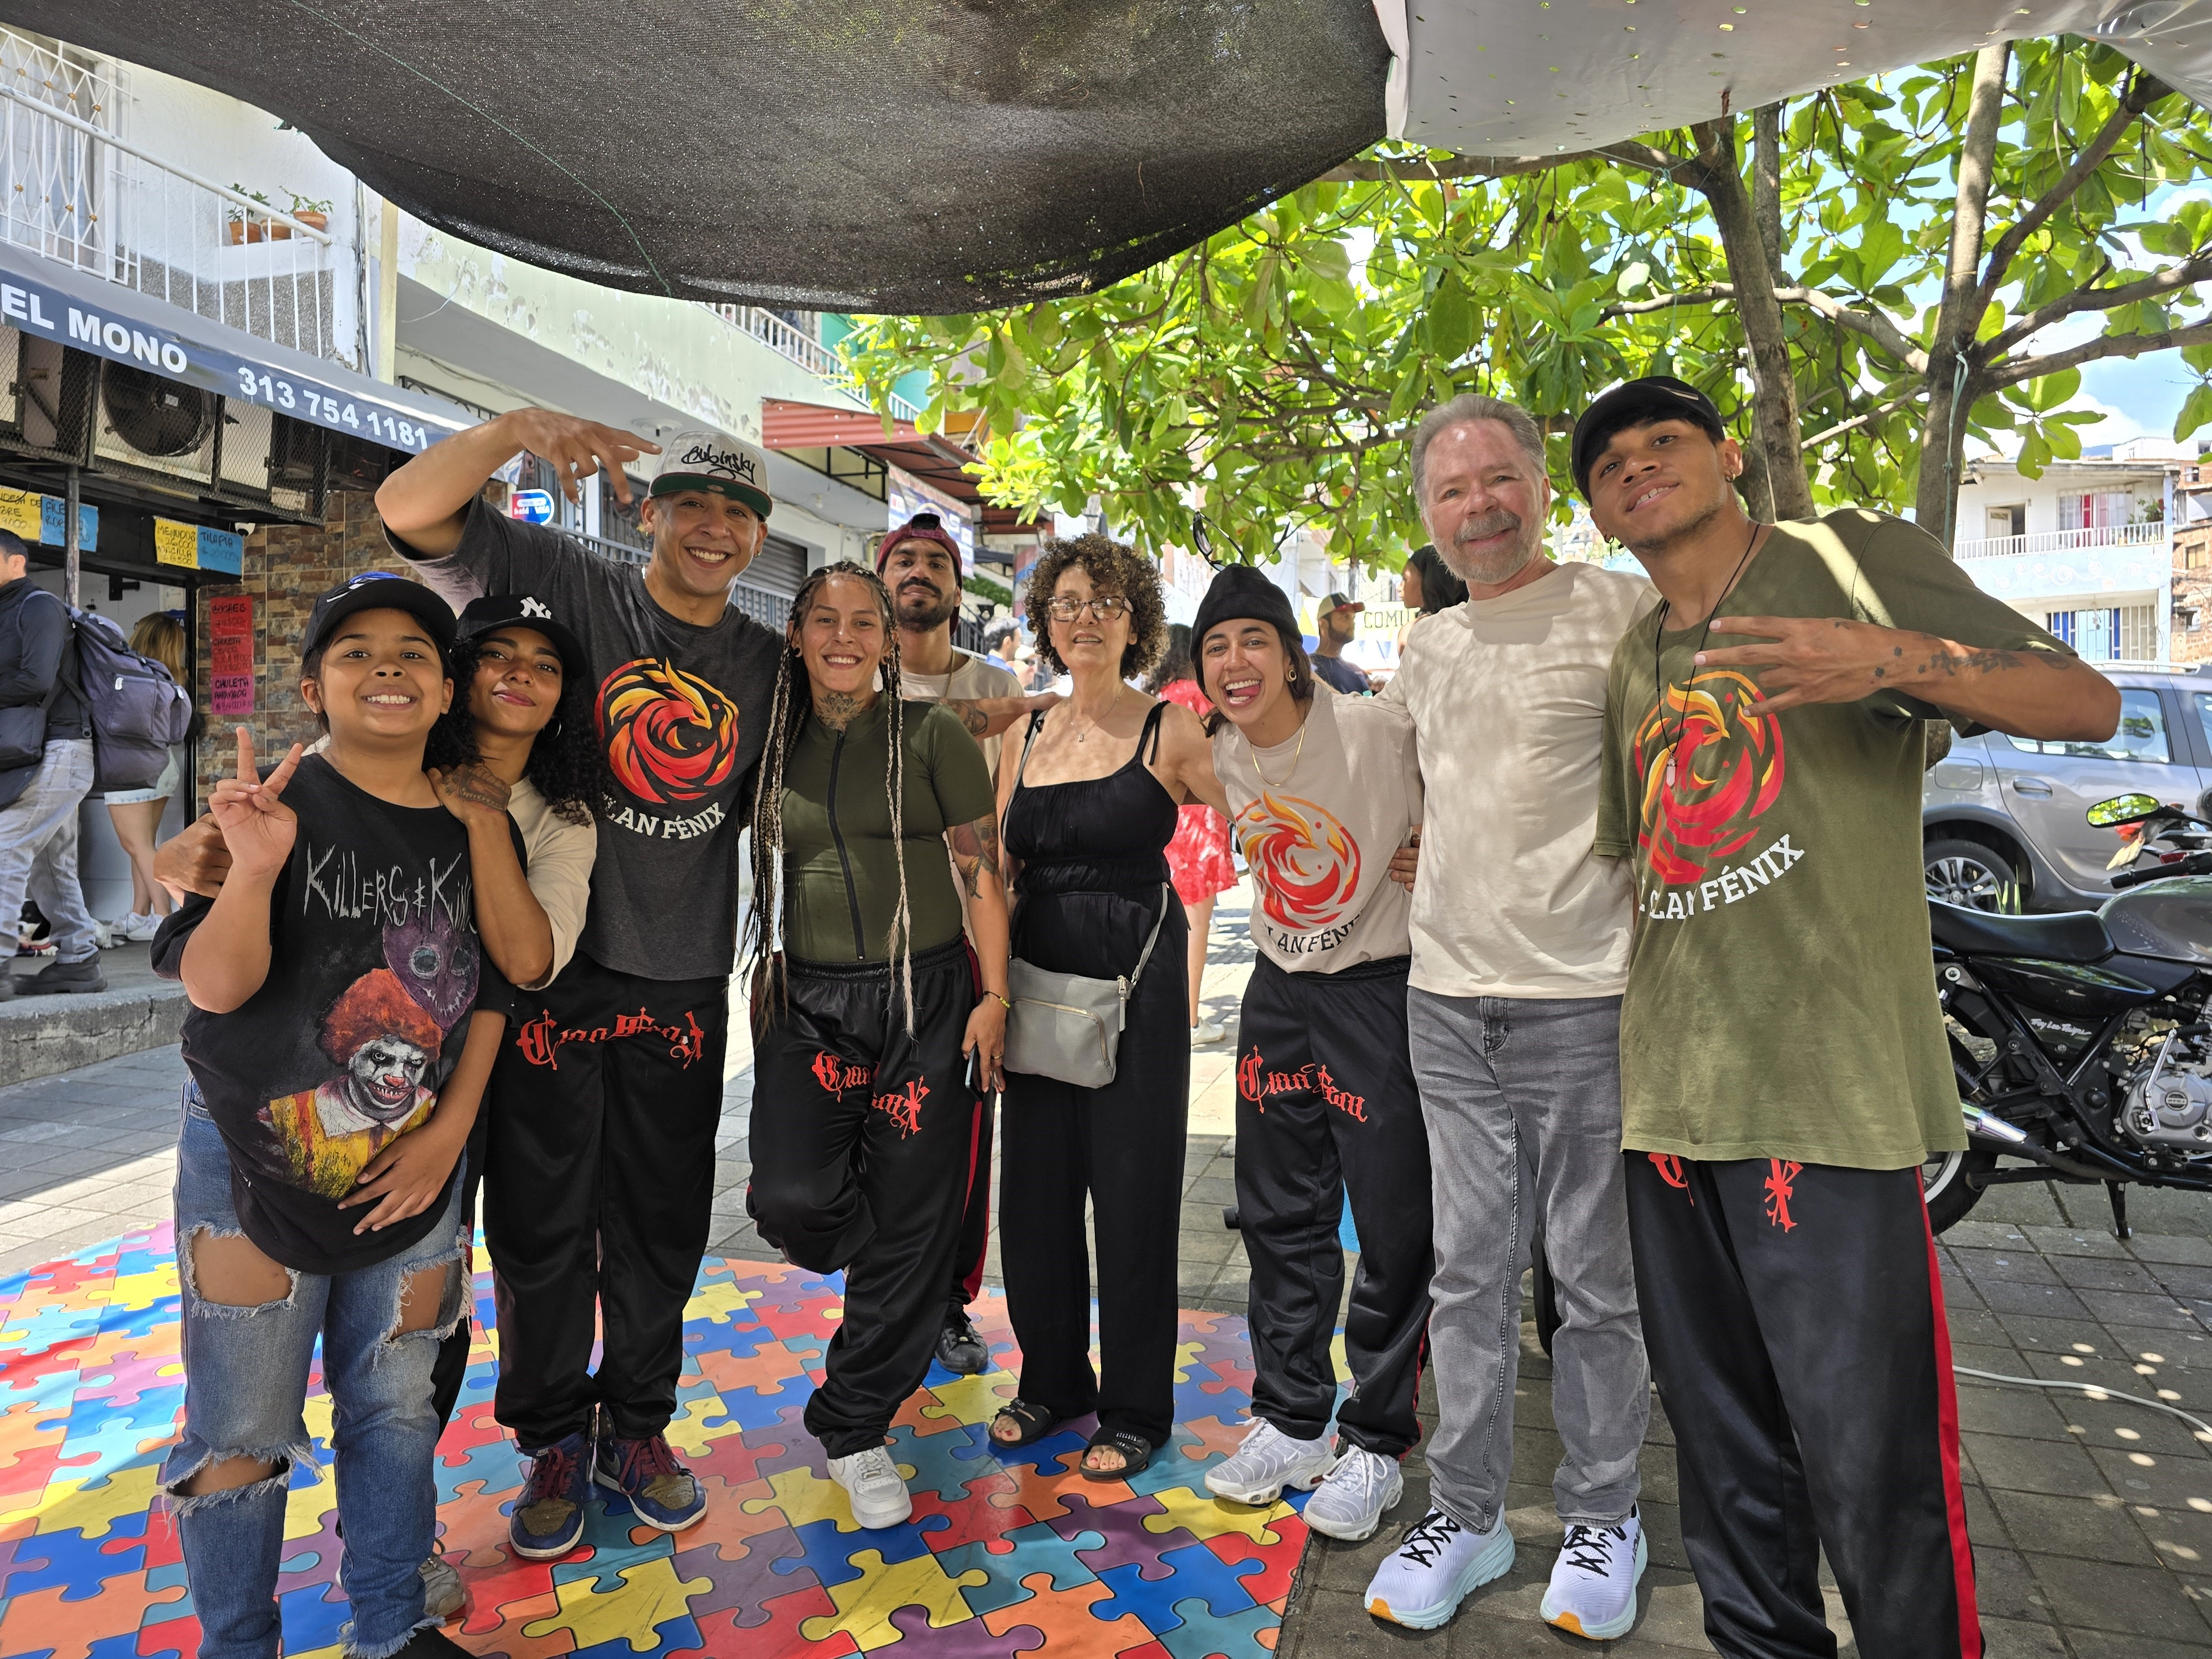
\includegraphics[width=0.15\linewidth]{dancers} \includegraphics[width=0.15\linewidth]{trail} 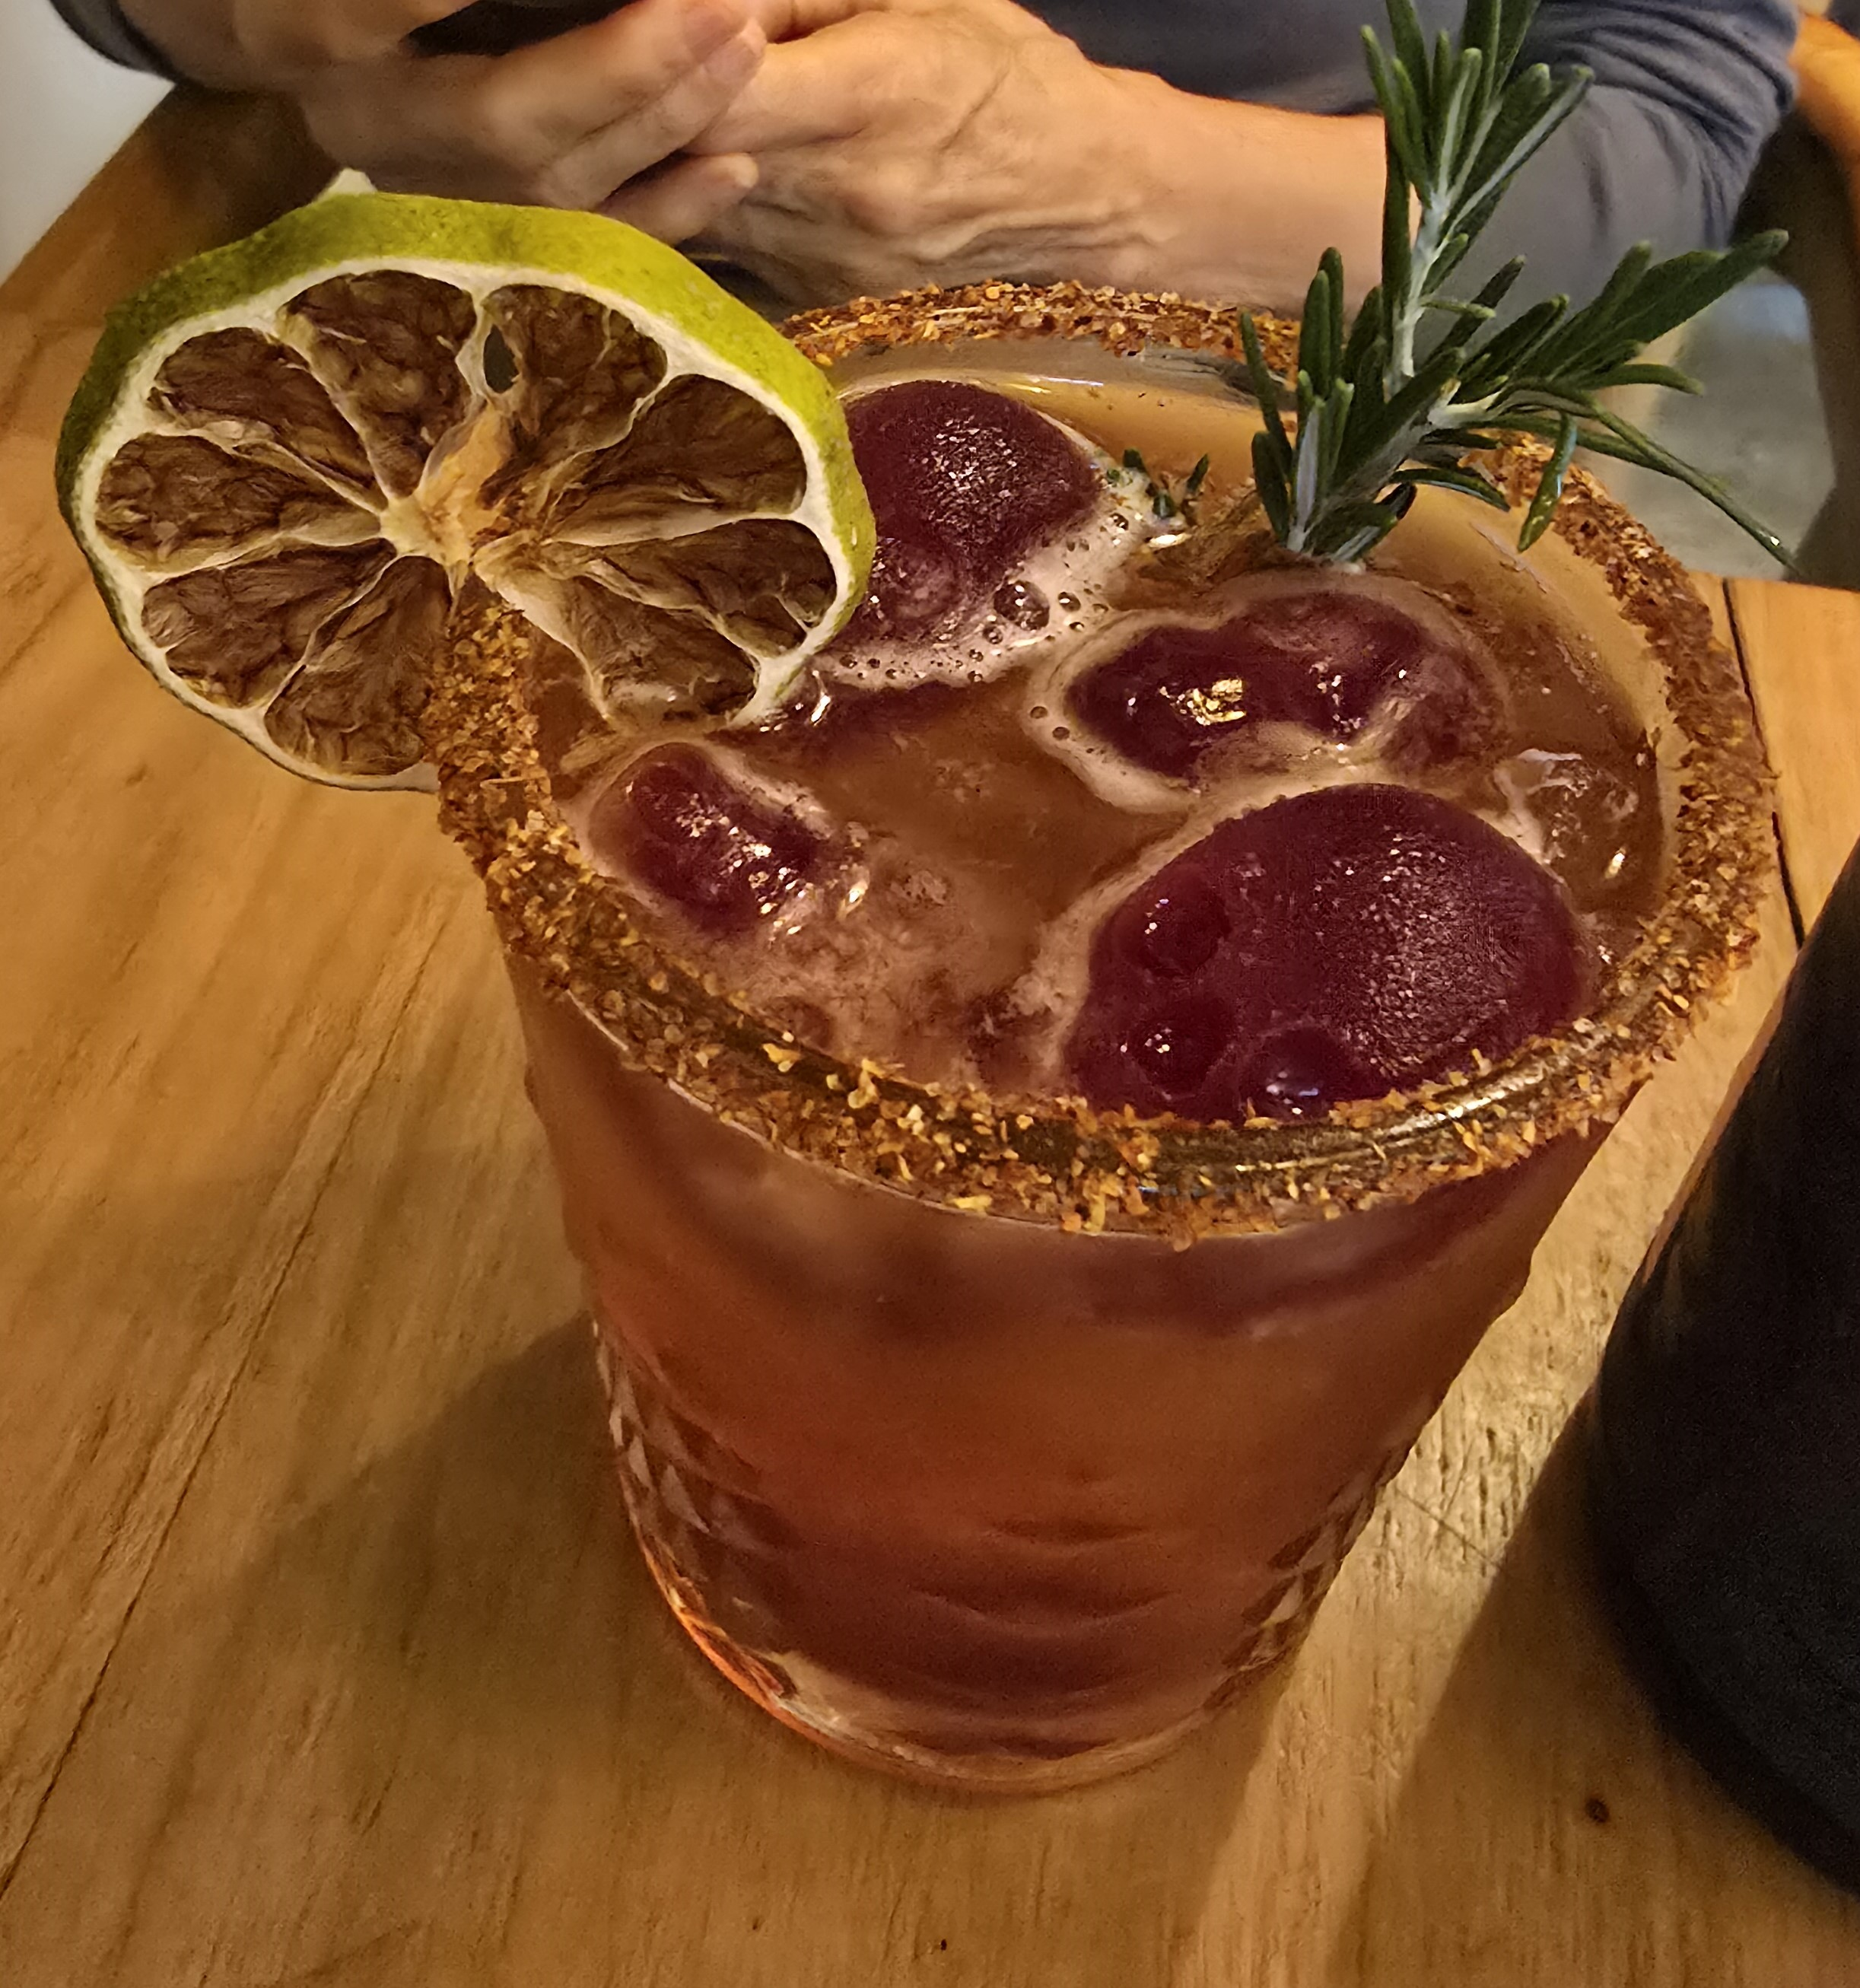
\includegraphics[width=0.15\linewidth]{drink} 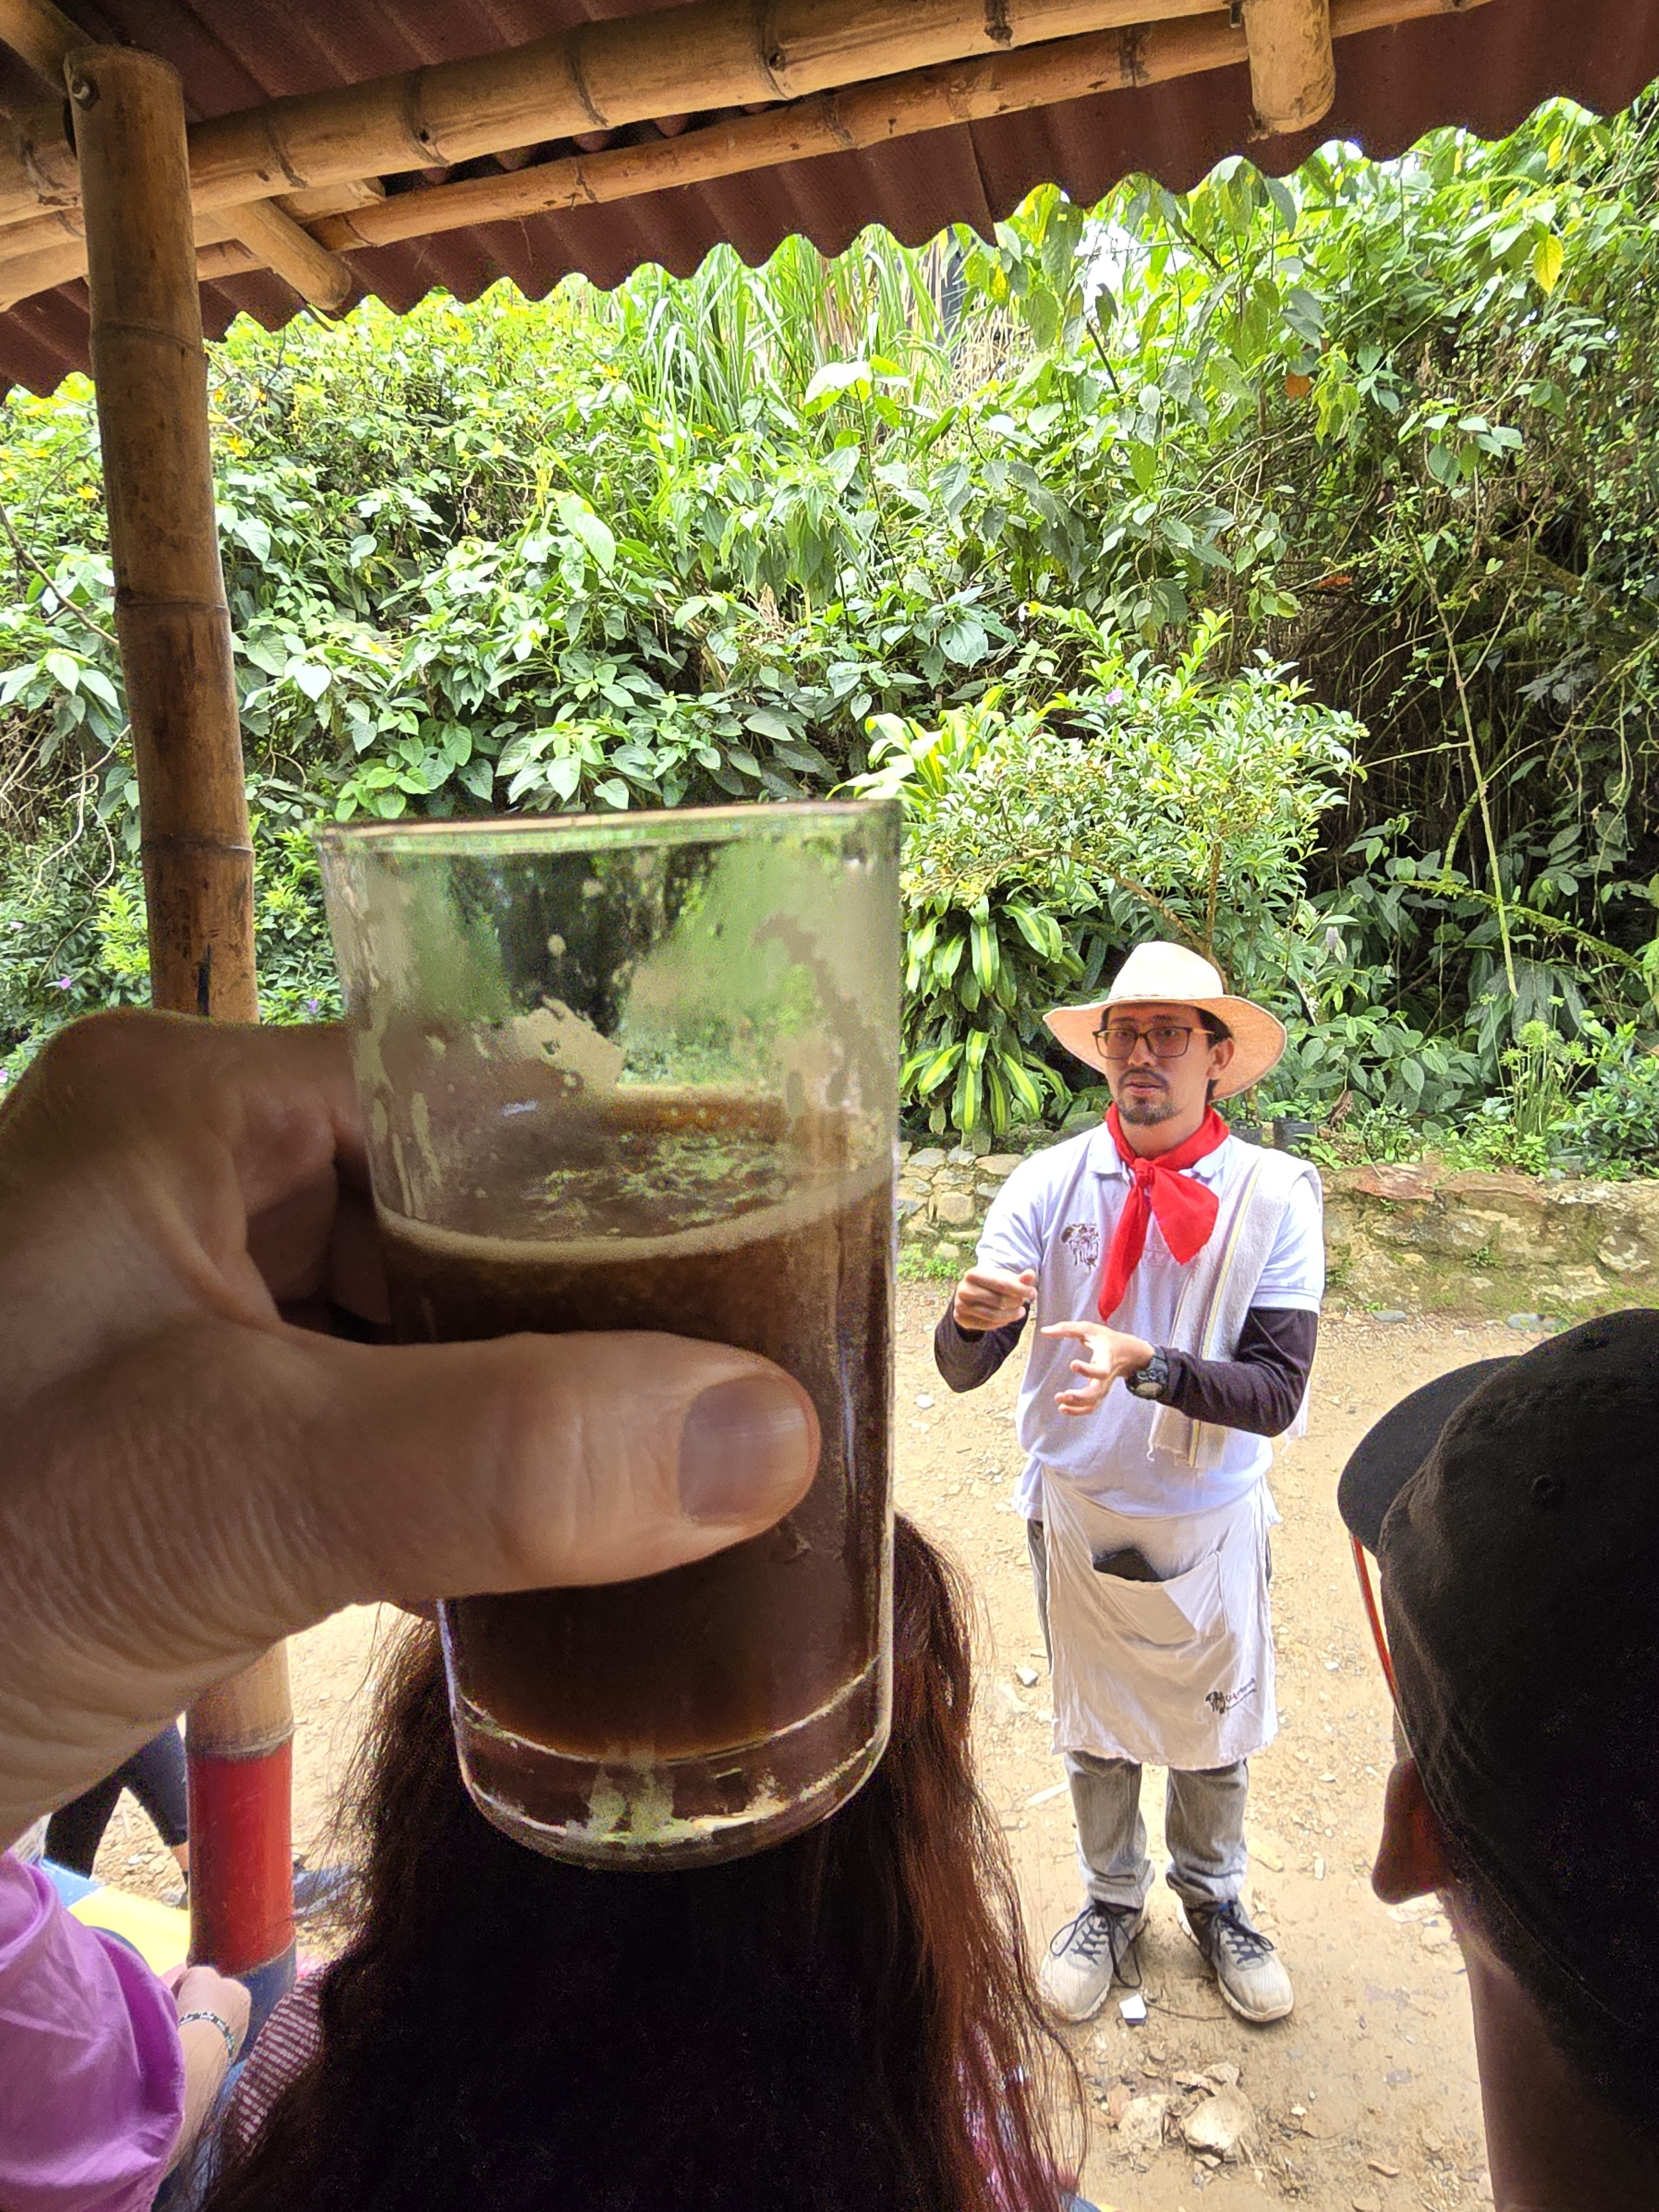
\includegraphics[width=0.15\linewidth]{coffee4} 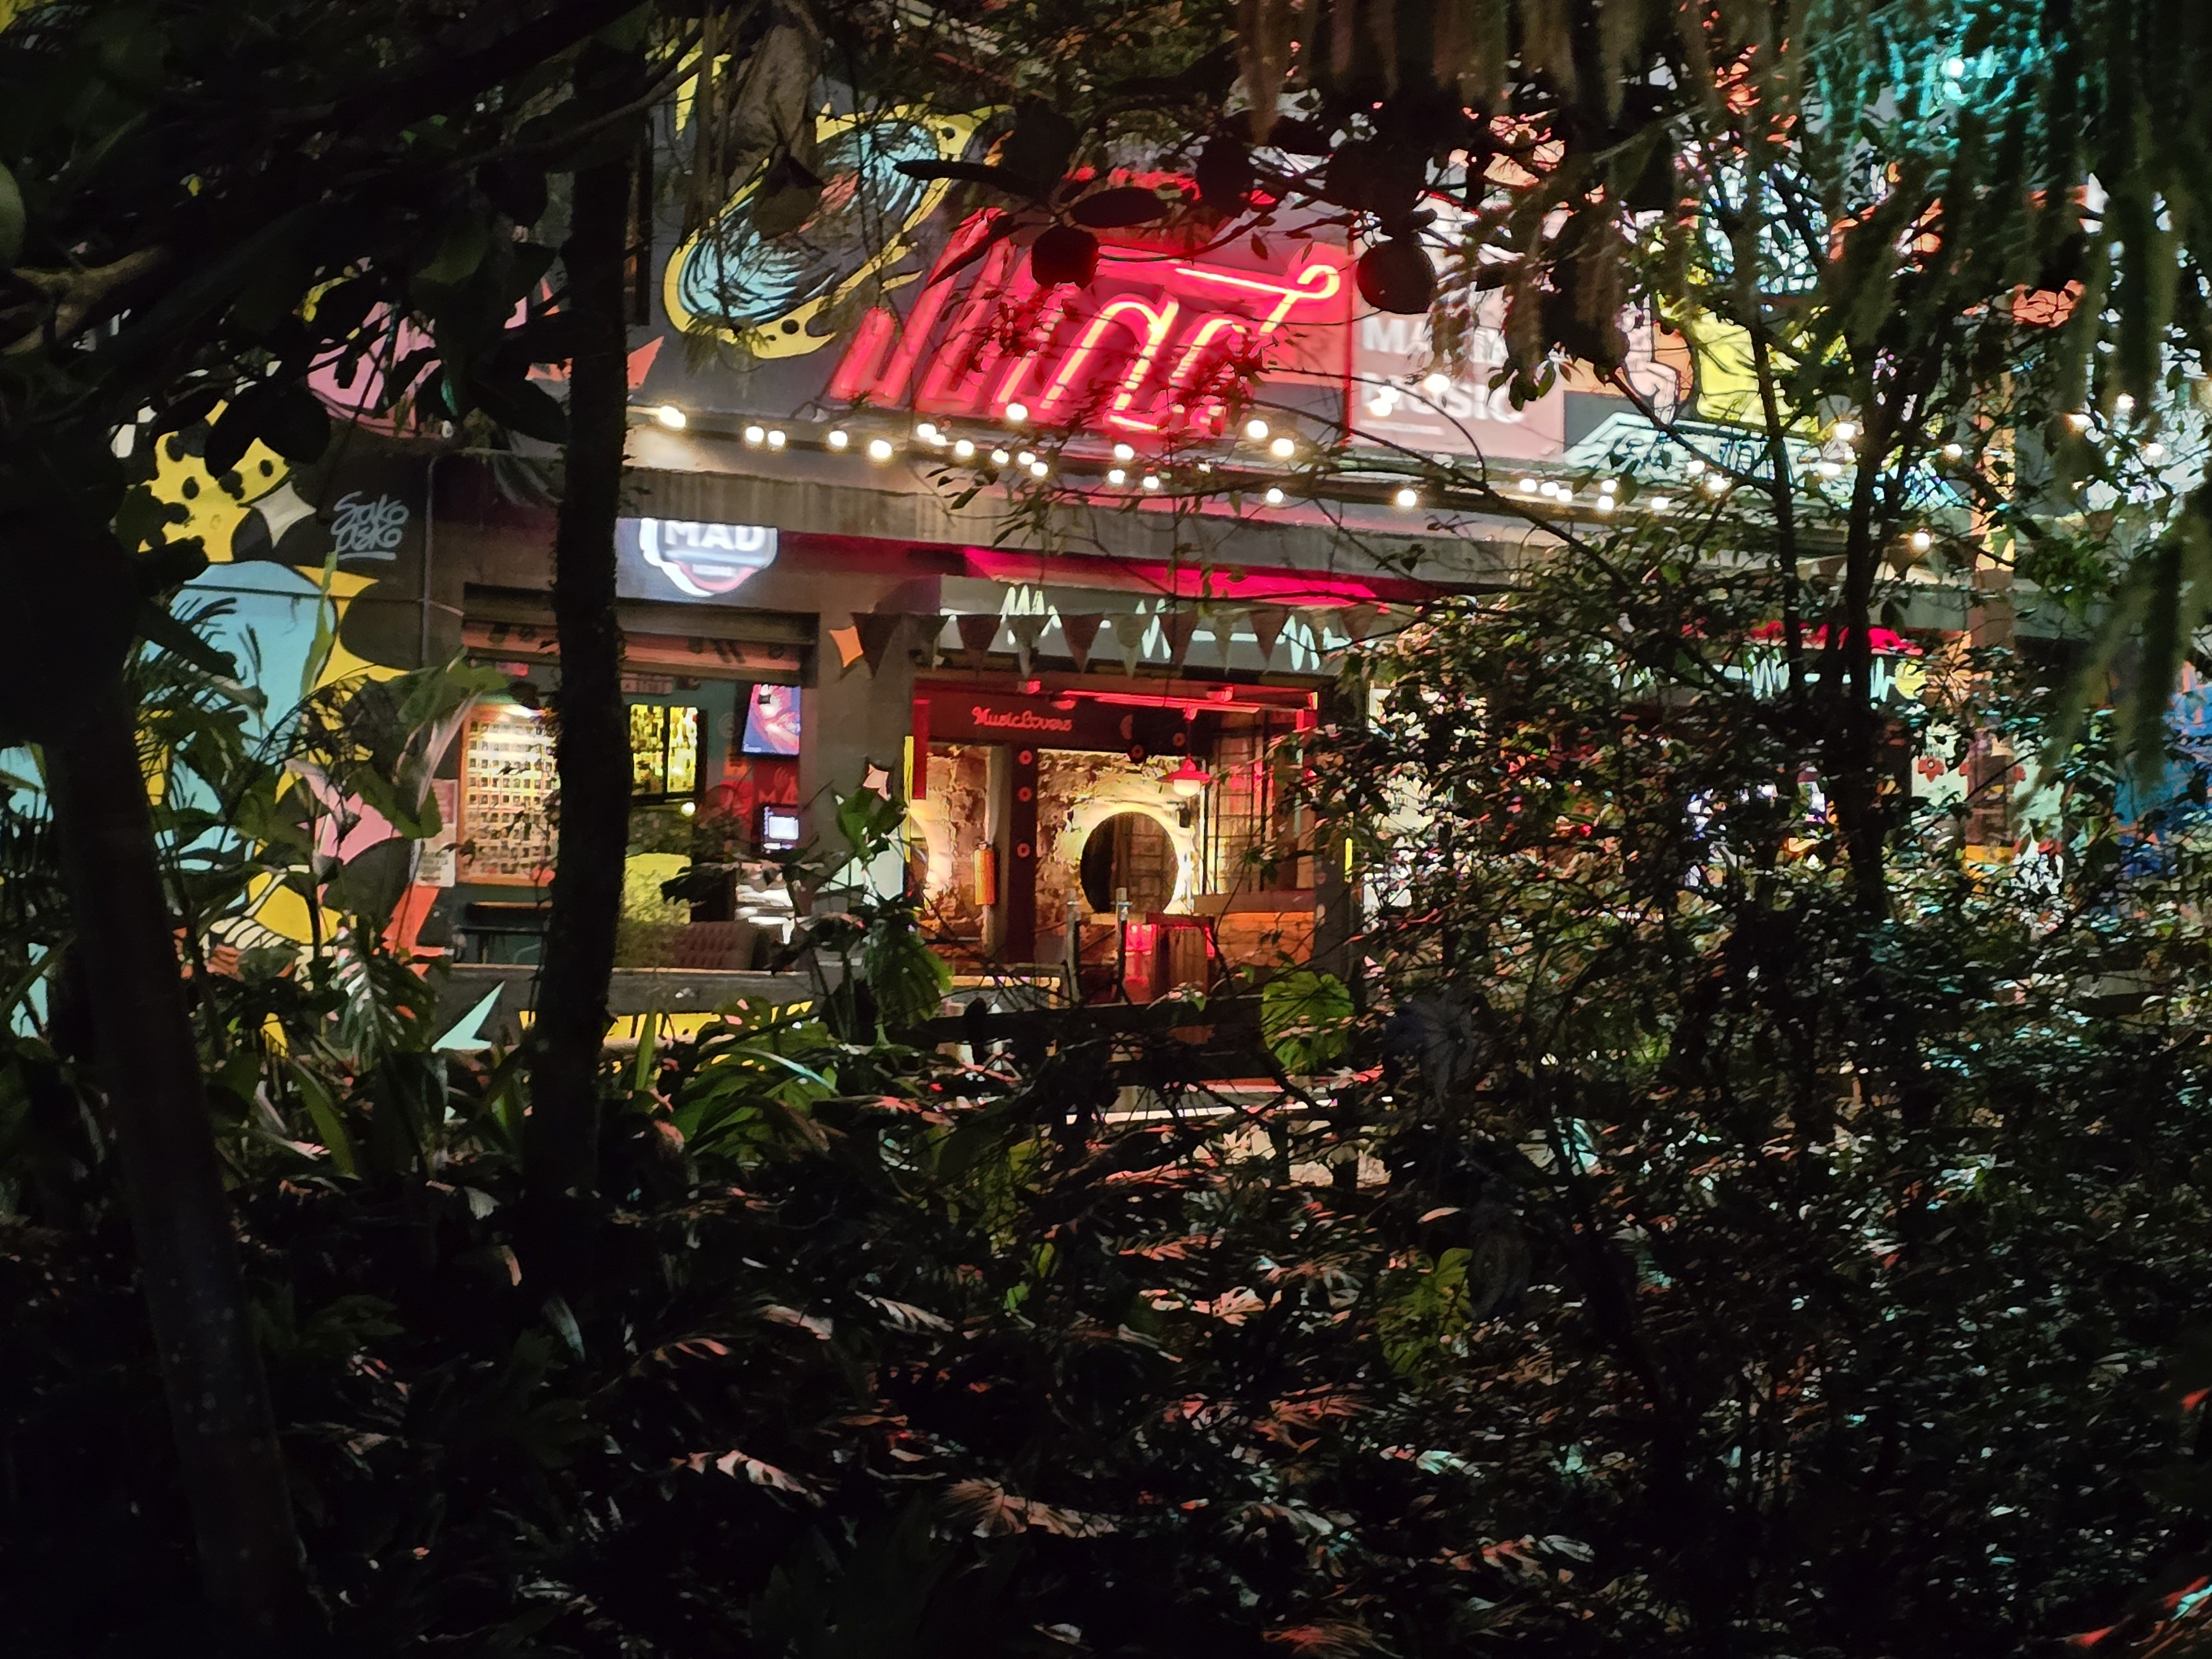
\includegraphics[width=0.15\linewidth]{el_pueblo} 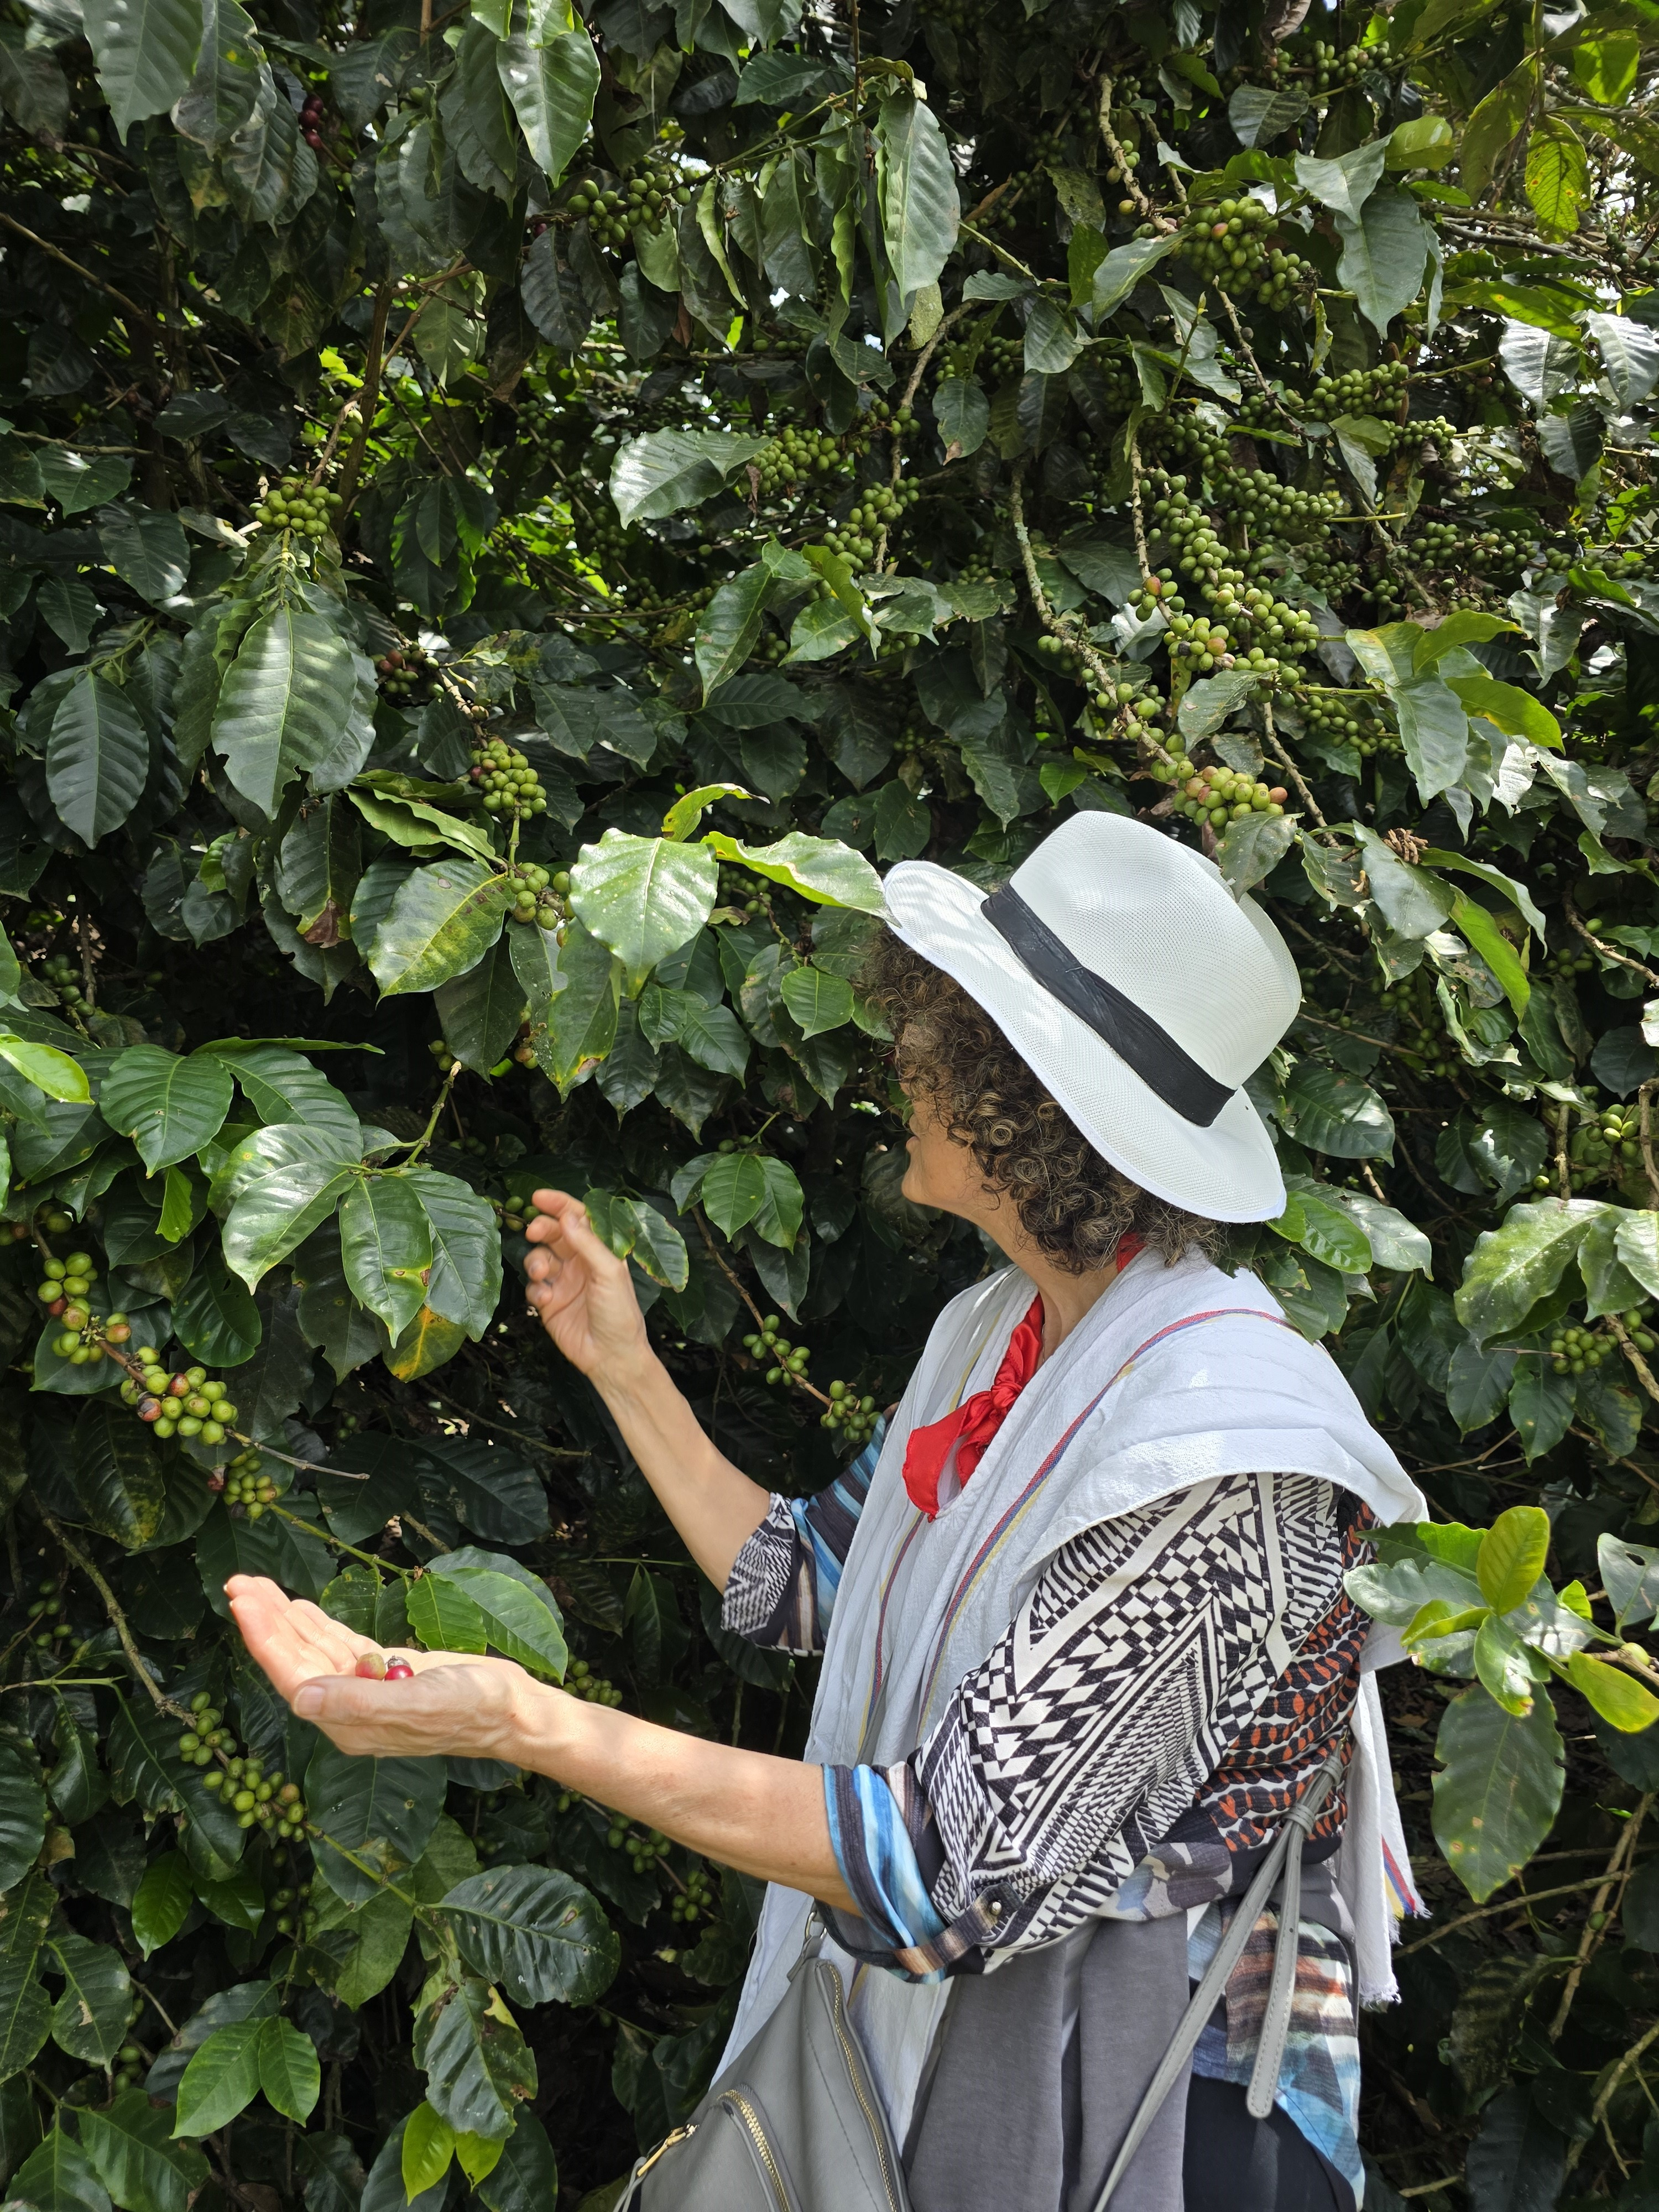
\includegraphics[width=0.15\linewidth]{randacoffee2} 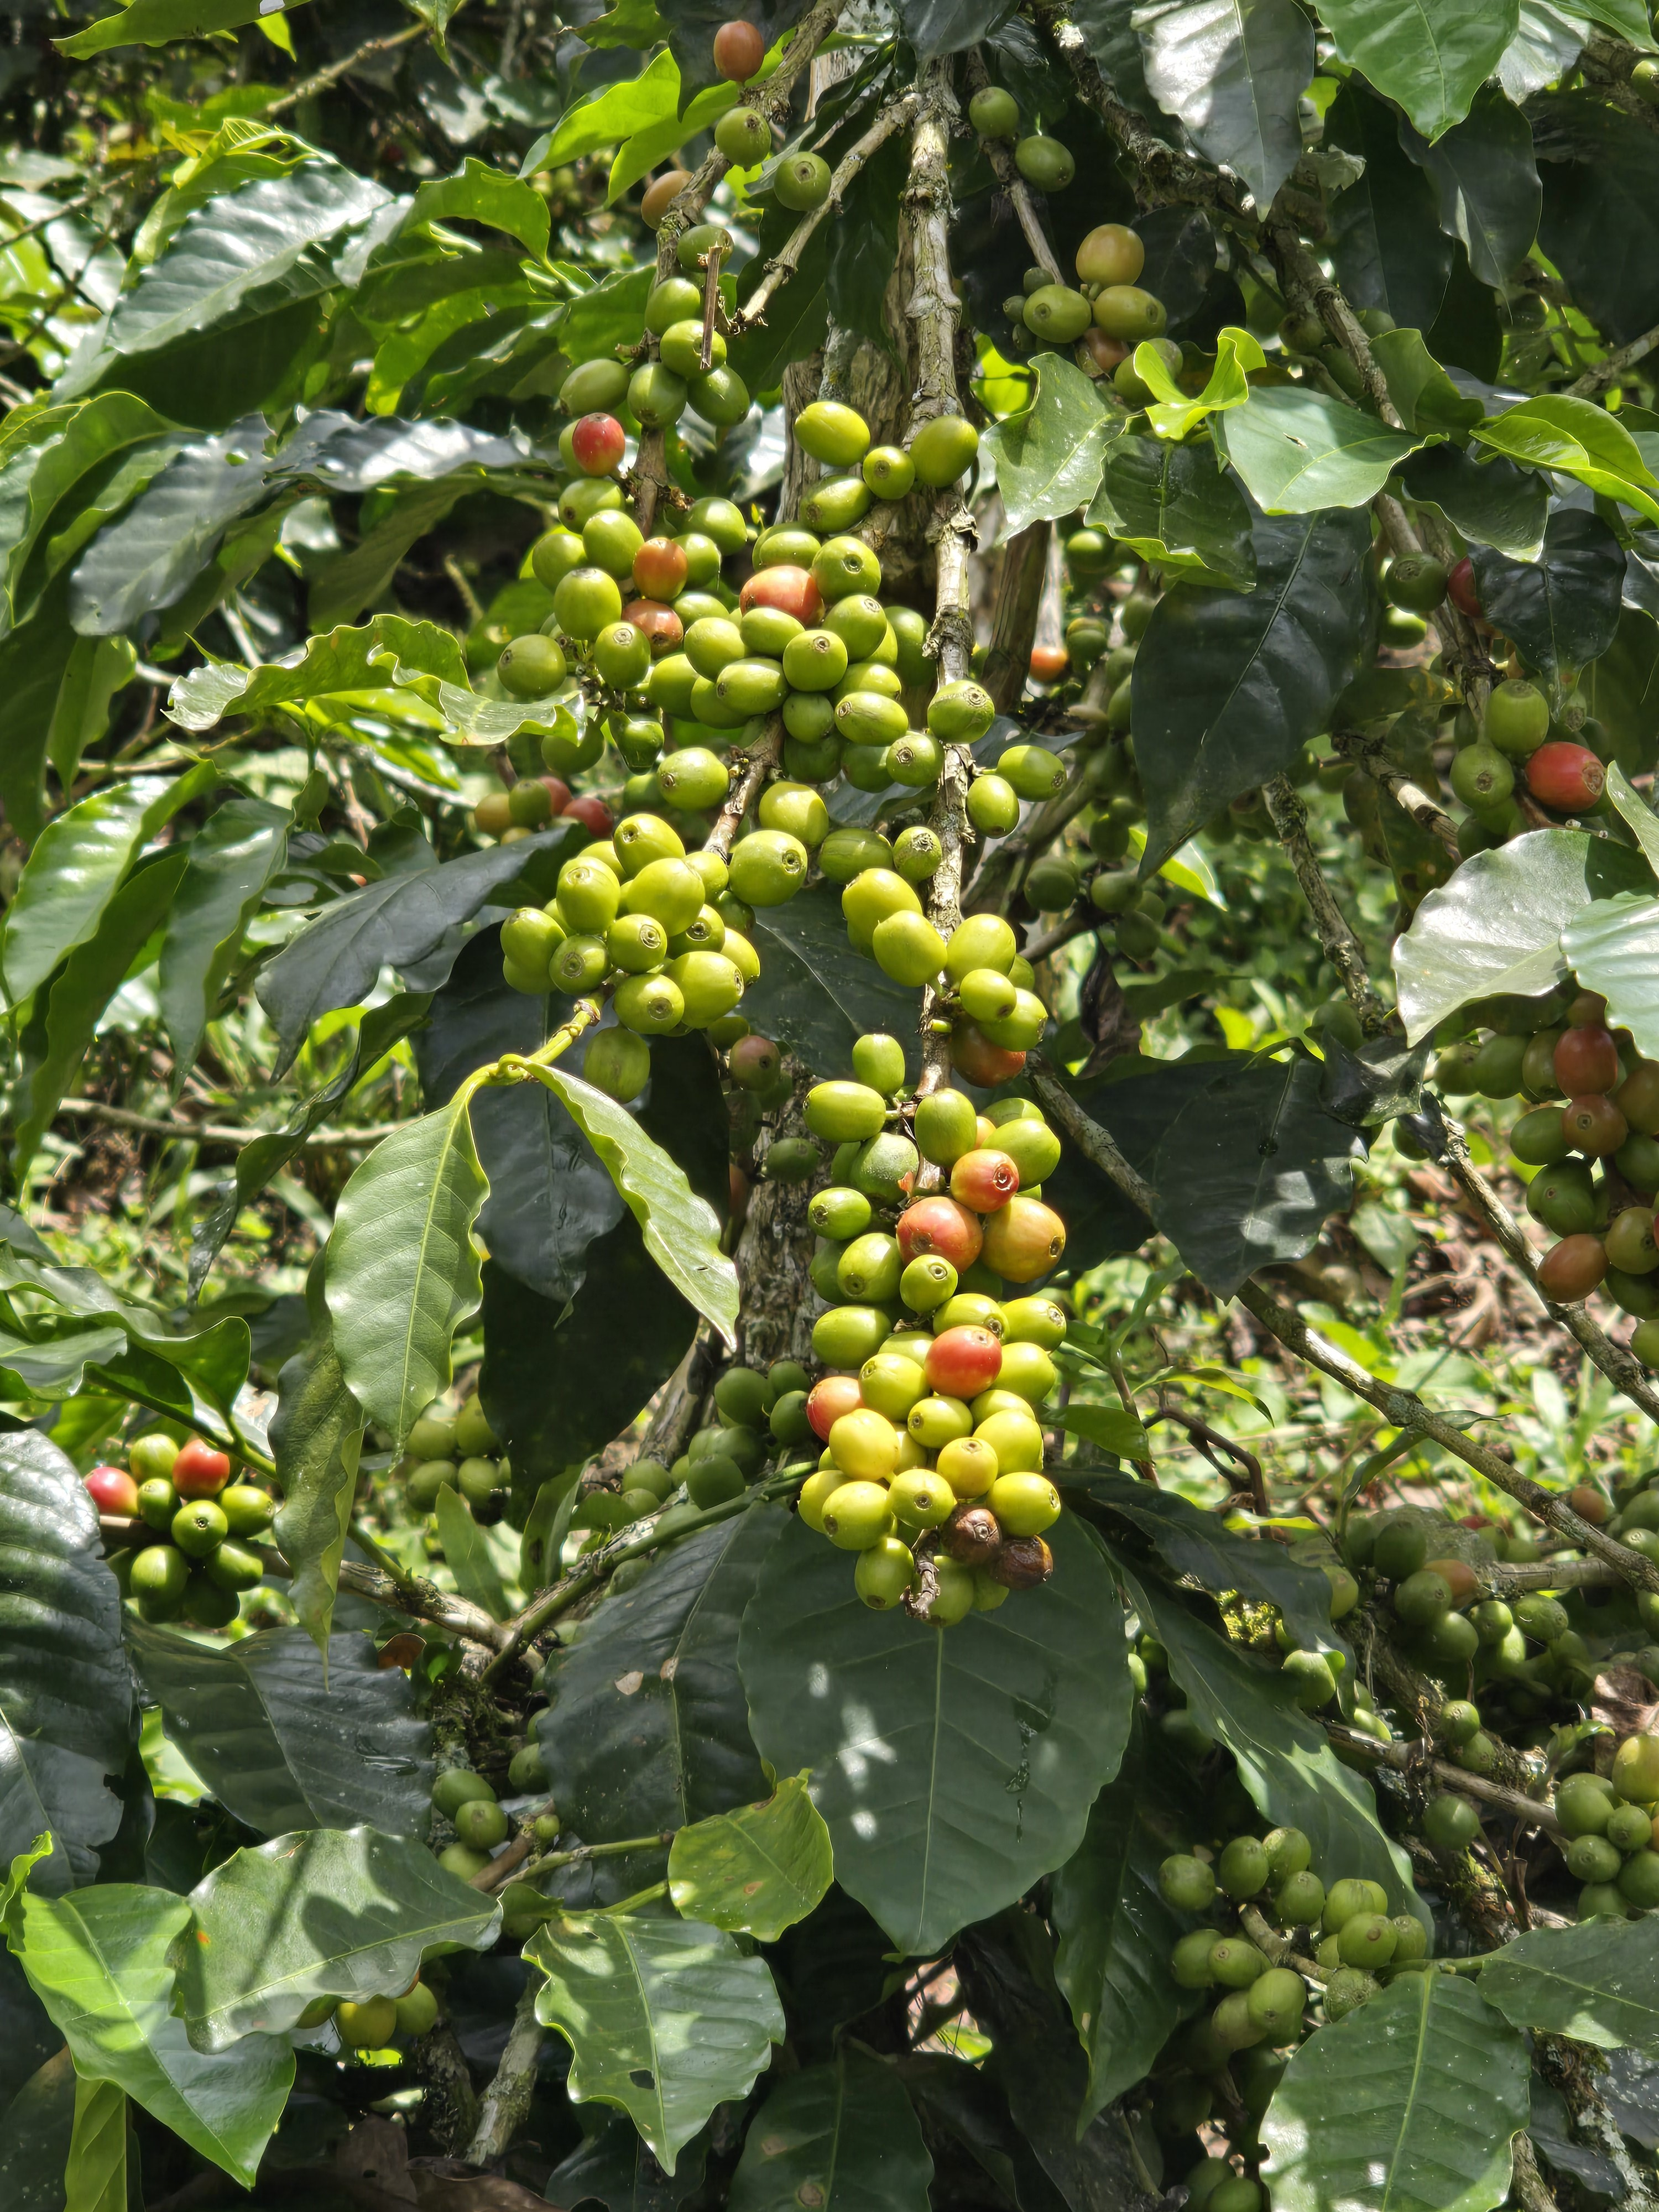
\includegraphics[width=0.15\linewidth]{coffee2} 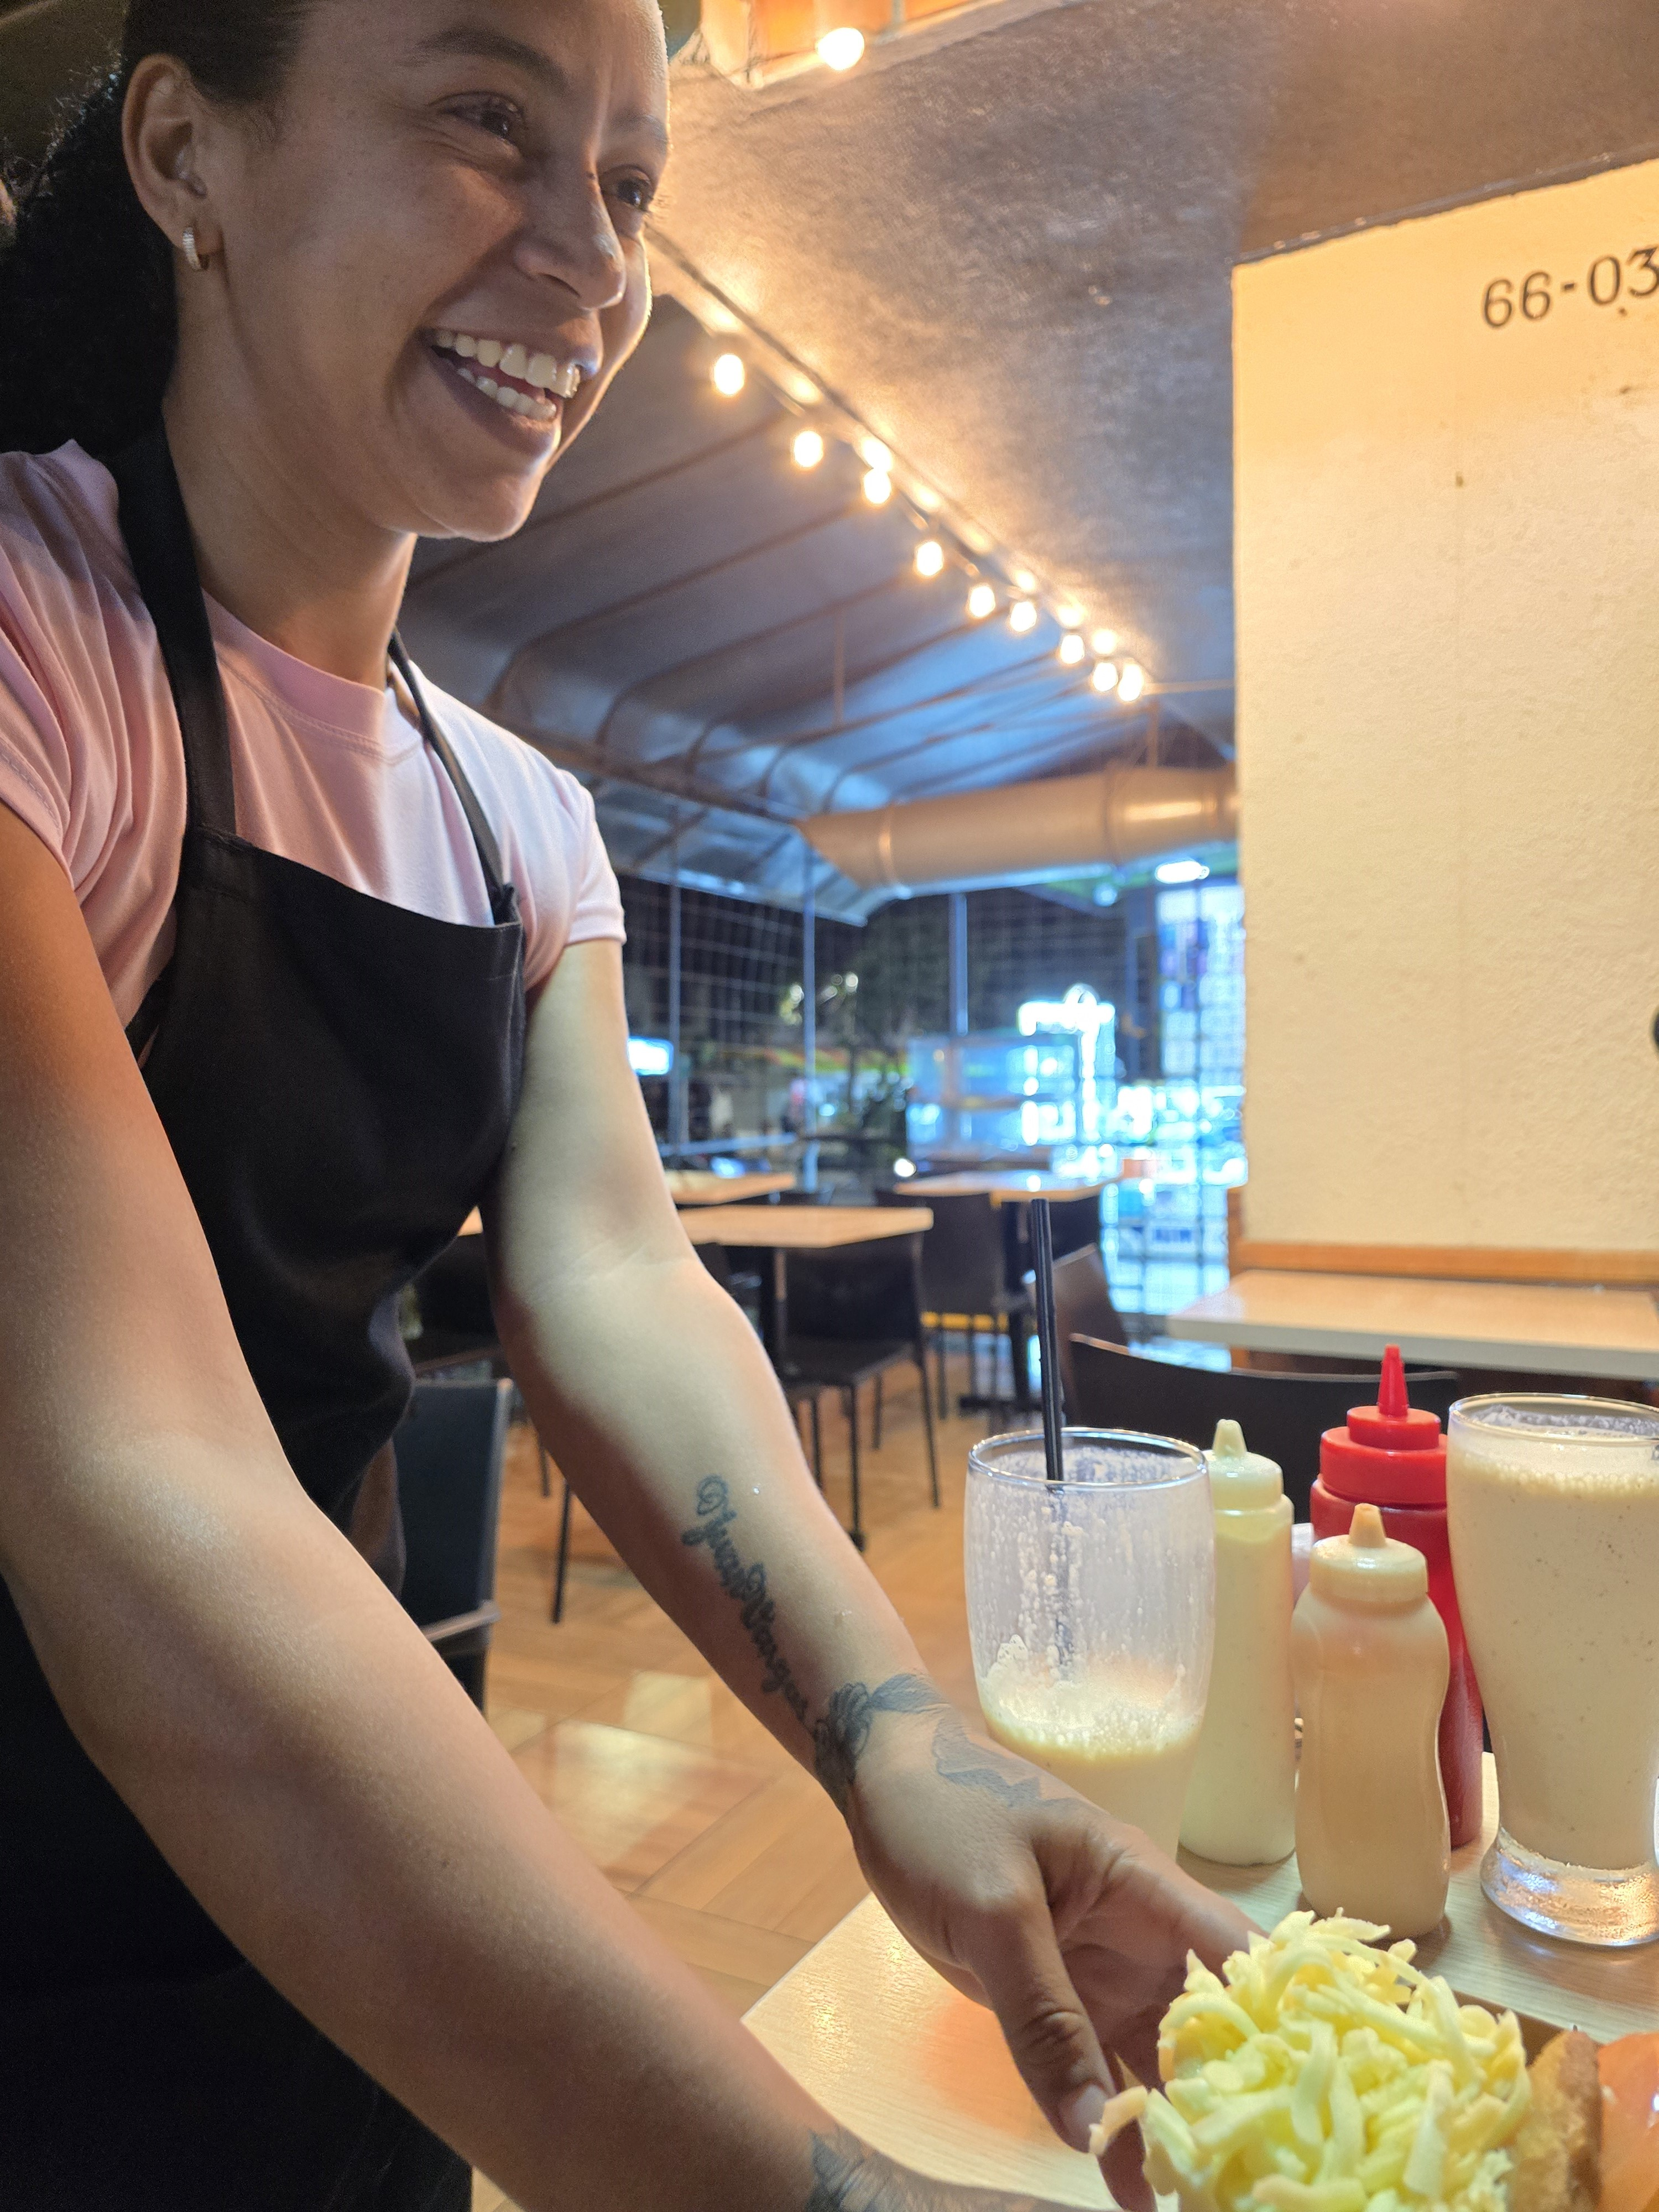
\includegraphics[width=0.15\linewidth]{arepa3} \end{center}
\end{frame}

\begin{frame}{Reflection}
\phantomsection\label{reflection}
\begin{center}\includegraphics[width=0.45\linewidth]{universe} \includegraphics[width=0.45\linewidth]{sitelink} \end{center}
\end{frame}

\end{document}
